\section{Internal ILD integration}
%\writer{Karsten Buesser, Roman Poeschl, Toshiaki Tauchi}{3}

The ILD detector concept underwent a dedicated effort to come to an integrated design that from subdetector level up to the major structures gives a conceptual engineering view of the full system. This includes realistic mechanical designs with tolerances, deformations and dead material zones as well as an integrated design of all detector services: electrical, cooling, gases, etc.

\subsection{ILD Mechanical Structure}

The mechanical structure of ILD has not changed since the DBD~\cite{ild:bib:ilddbd}. The main parts are the three barrel yoke rings and the two endcaps. The central barrel ring carries the solenoid coil in its cryostat; all barrel detectors are suspended from the cryostat. The two other central yoke rings can move over the cryostat. The endcaps can be opened as well. All rings can be moved using airpad systems. Figure~\ref{ILD:fig:mechanical_model} shows the mechanical model of the ILD yoke structure.
\begin{figure}[h!]
    \centering
    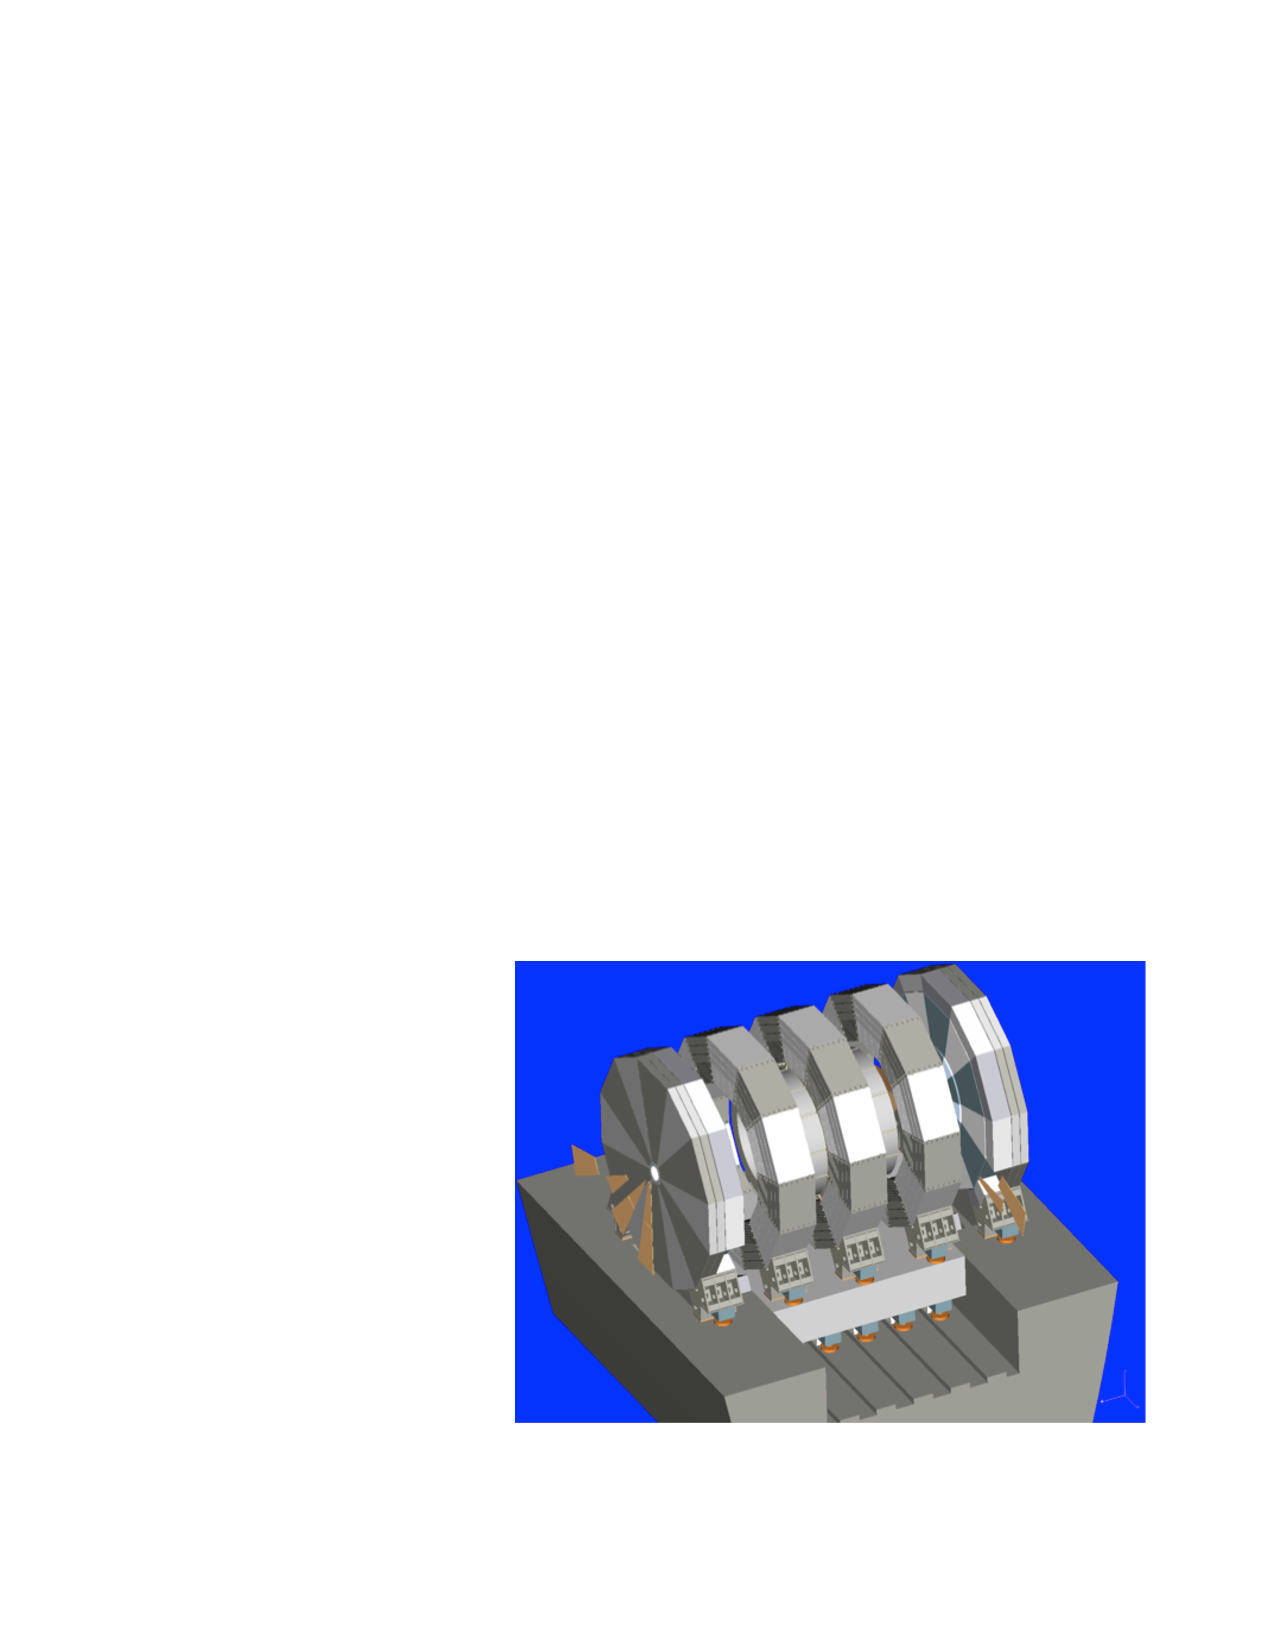
\includegraphics[width=1.0\hsize]{Integration/fig/ILD_Mechanical.pdf}
    \caption{Mechanical structure of the ILD detector~\cite{ild:bib:ilddbd}.}
    \label{ILD:fig:mechanical_model}
\end{figure}


\subsection{ILD Services and Utilities}
\label{ild:sec:services}
Each component of ILD has requirements on services and utilities that are needed for operations and maintenance. This typically includes power and data lines, gas and cooling systems, guidances for laser beams, etc. All major support systems for those services, e.g. power supplies, cooling plants, lasers, DAQ computers, or gas systems are located outside of the detector, sometimes even far away (c.f.~section~\ref{ild:sec:service_locations}). General paths have been defined in the global detector structure where space is allocated for those services. The routing of those paths has to be designed to minimise the amount of gaps and dead material in the active detector areas, while at the same time provide enough space for the foreseen utilities. Three main pathways have been defined for ILD:
\begin{enumerate}
    \item The services of all barrel detectors are collected at both front-faces of the barrel, go around the solenoid cryostat and leave the detector through the gap between the central yoke ring and the neighbouring rings.
    \item The services of the endcap detectors (ECAL, HCAL, Muon) leave the detector along the endcap yoke ring.
    \item The services for the forward calorimeter systems (FCAL, ECAL ring) pass parallel to the beamline, outside of the QD0 magnet.
\end{enumerate}

This scheme allows for the opening of the yoke endcaps as well as for moving the barrel yoke rings independently from each other. The front-end electronic systems of the subdetectors can often drive only a limited cable length. Therefore, space for additional patch panels, drivers, data concentrators needs to be provided inside the ILD detector. While the exact requirements for those are not known in each case, conceptual locations have been defined. Figure~\ref{ILD:fig:cable_paths} shows the general service paths and proposed locations for the patch panels in ILD.

\begin{figure}[h!]
    \centering
    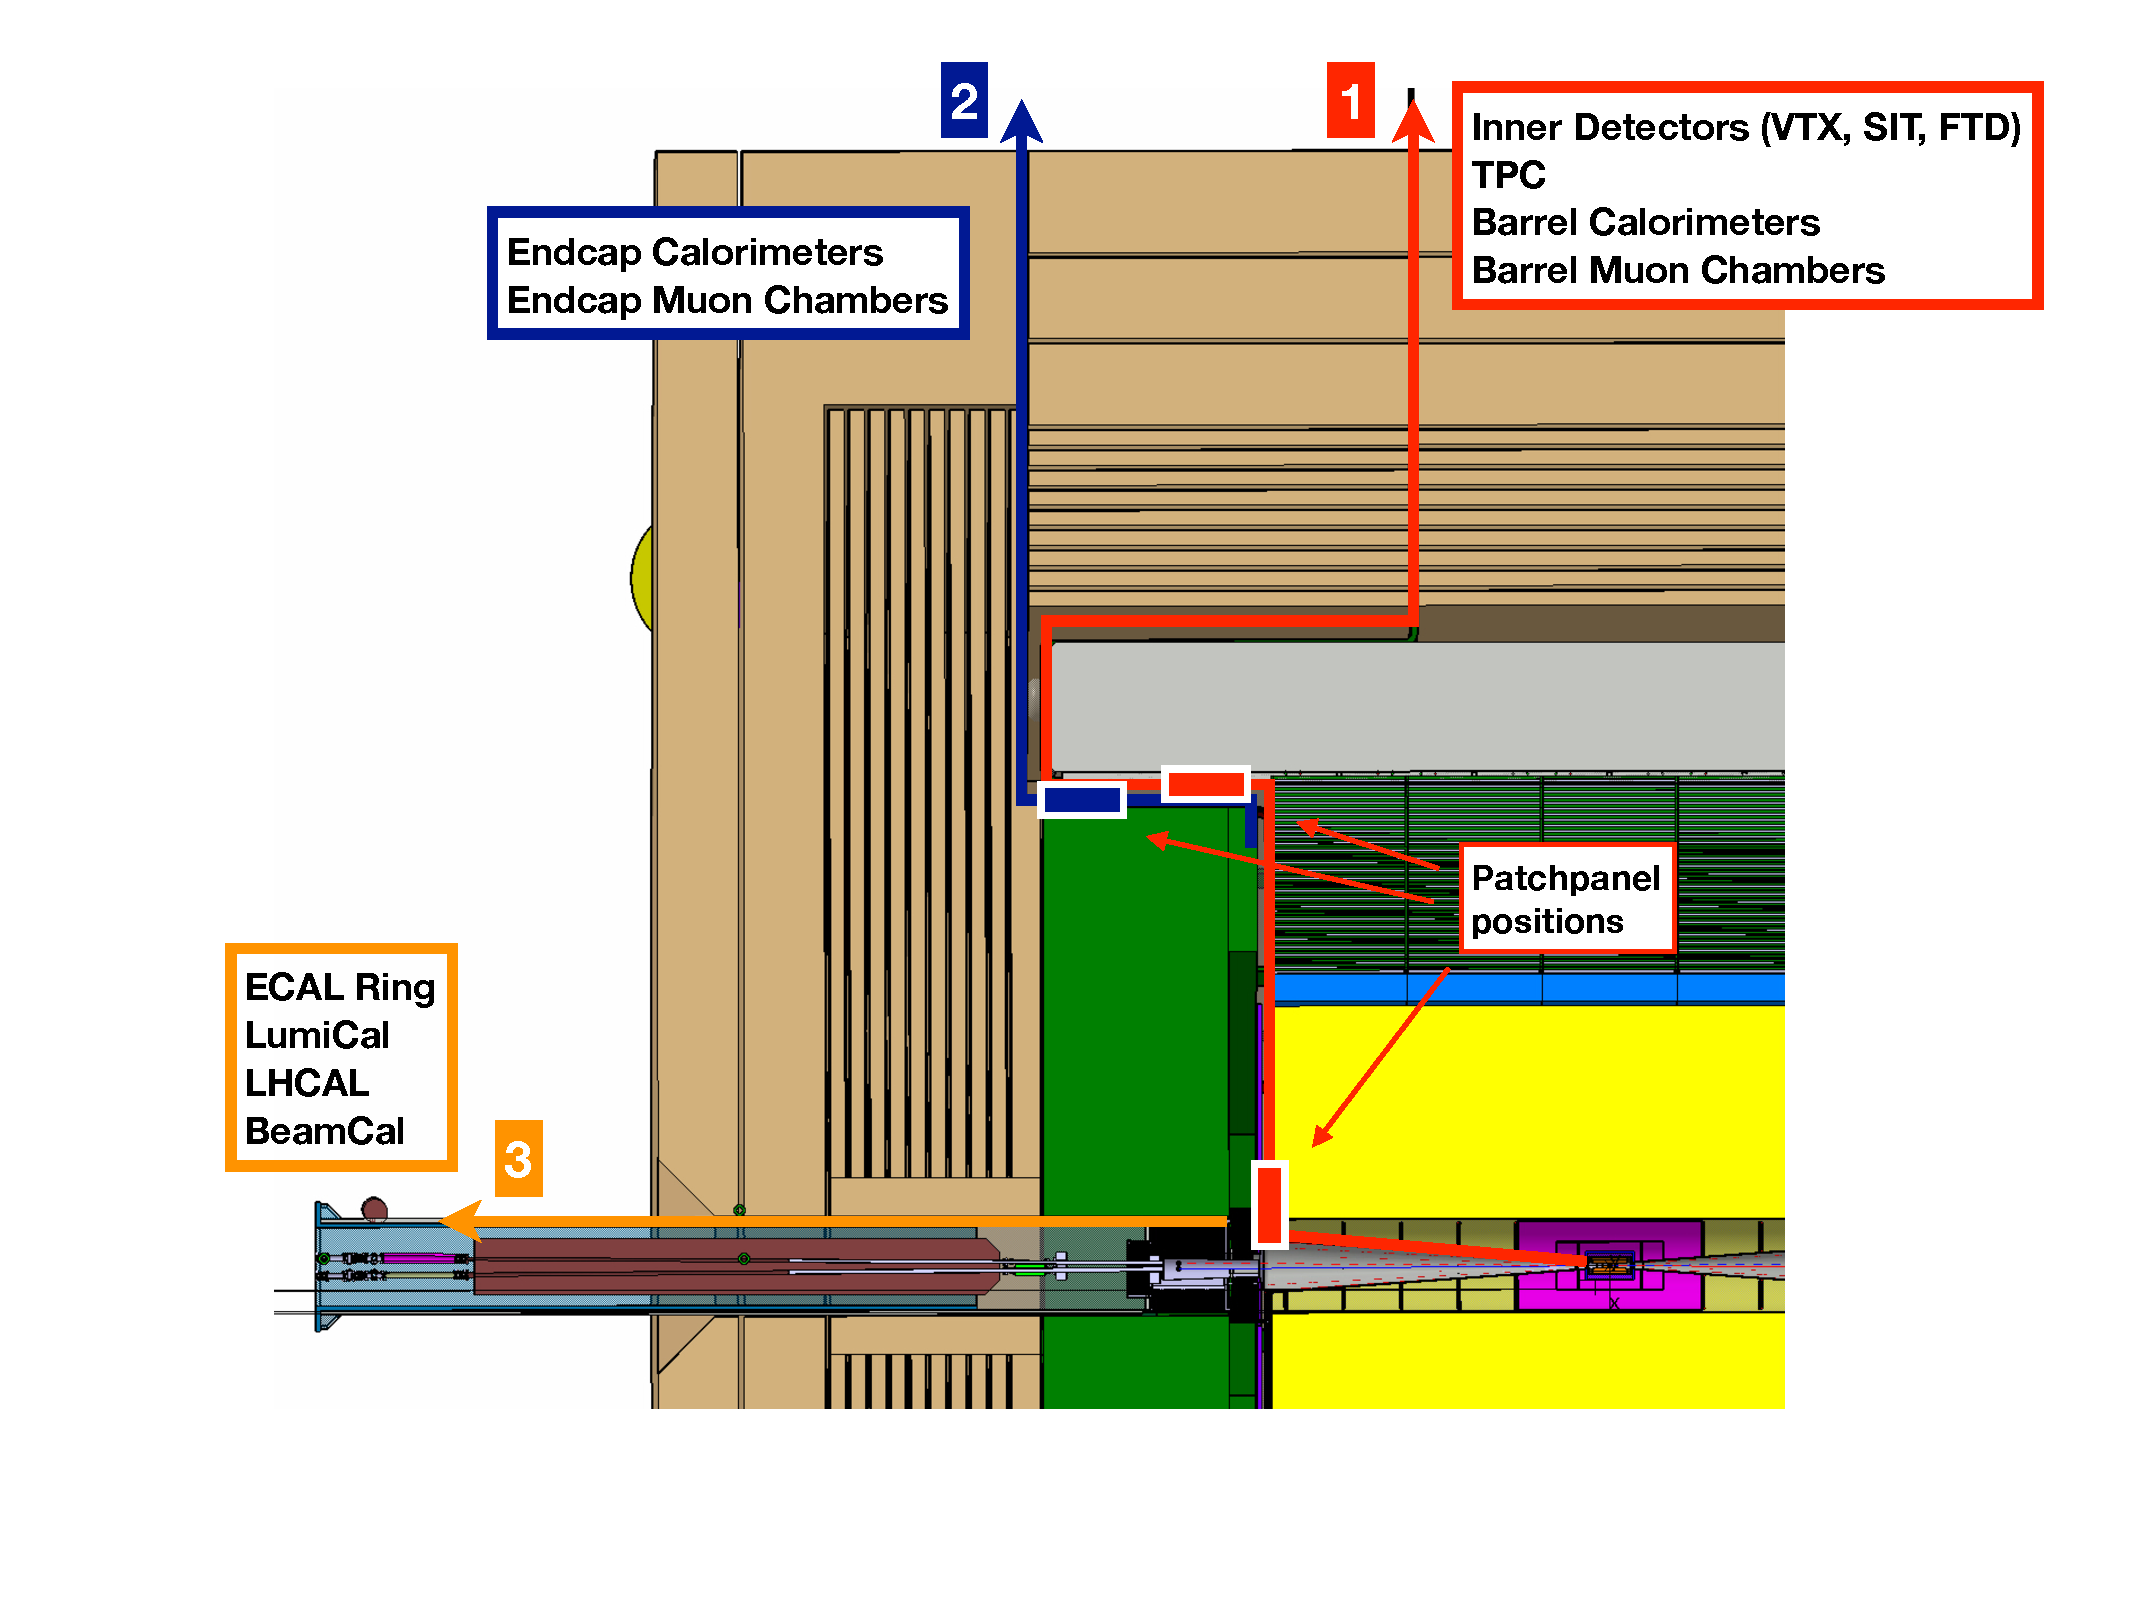
\includegraphics[width=1.0\hsize]{Integration/fig/cable_paths_new.pdf}
    \caption{Service paths in the ILD detector and suggested positions for patch panels.}
    \label{ILD:fig:cable_paths}
\end{figure}


\subsection{Inner Detector Integration}

At the heart of ILD, directly at the interaction point, is the inner detector that comprises the beam pipe as well as the vertex detector and the inner silicon tracking devices, SIT and FTD~(c.f.~Figure~\ref{ILD:fig:inner_detector_schematic}).

\subsubsection{Mechanical Integration}
The vertex detector is suspended from the beam pipe that itself is carried together with the Forward Tracking Disks and the Si Intermediate Tracker from the Inner Detector Support Structure (ISS). The ISS is a support tube made out of carbon-fibre reinforced plastic and is suspended from the end flanges of the TPC. A piezo-based active alignment system (see Figure~\ref{ILD:fig:inner_detector_integration}) allows for the positioning of the ISS with a precision better than 0.01~mm~\cite{ild:bib:inner_detector_integration}, independently of the main ILD detector structure. This is required to adjust the beam pipe and the inner tracking devices with respect to the beam axis, to better precision than what can be achieved with the complete ILD detector, e.g.~after push-pull operations.

\begin{figure}[h!]
    \centering
        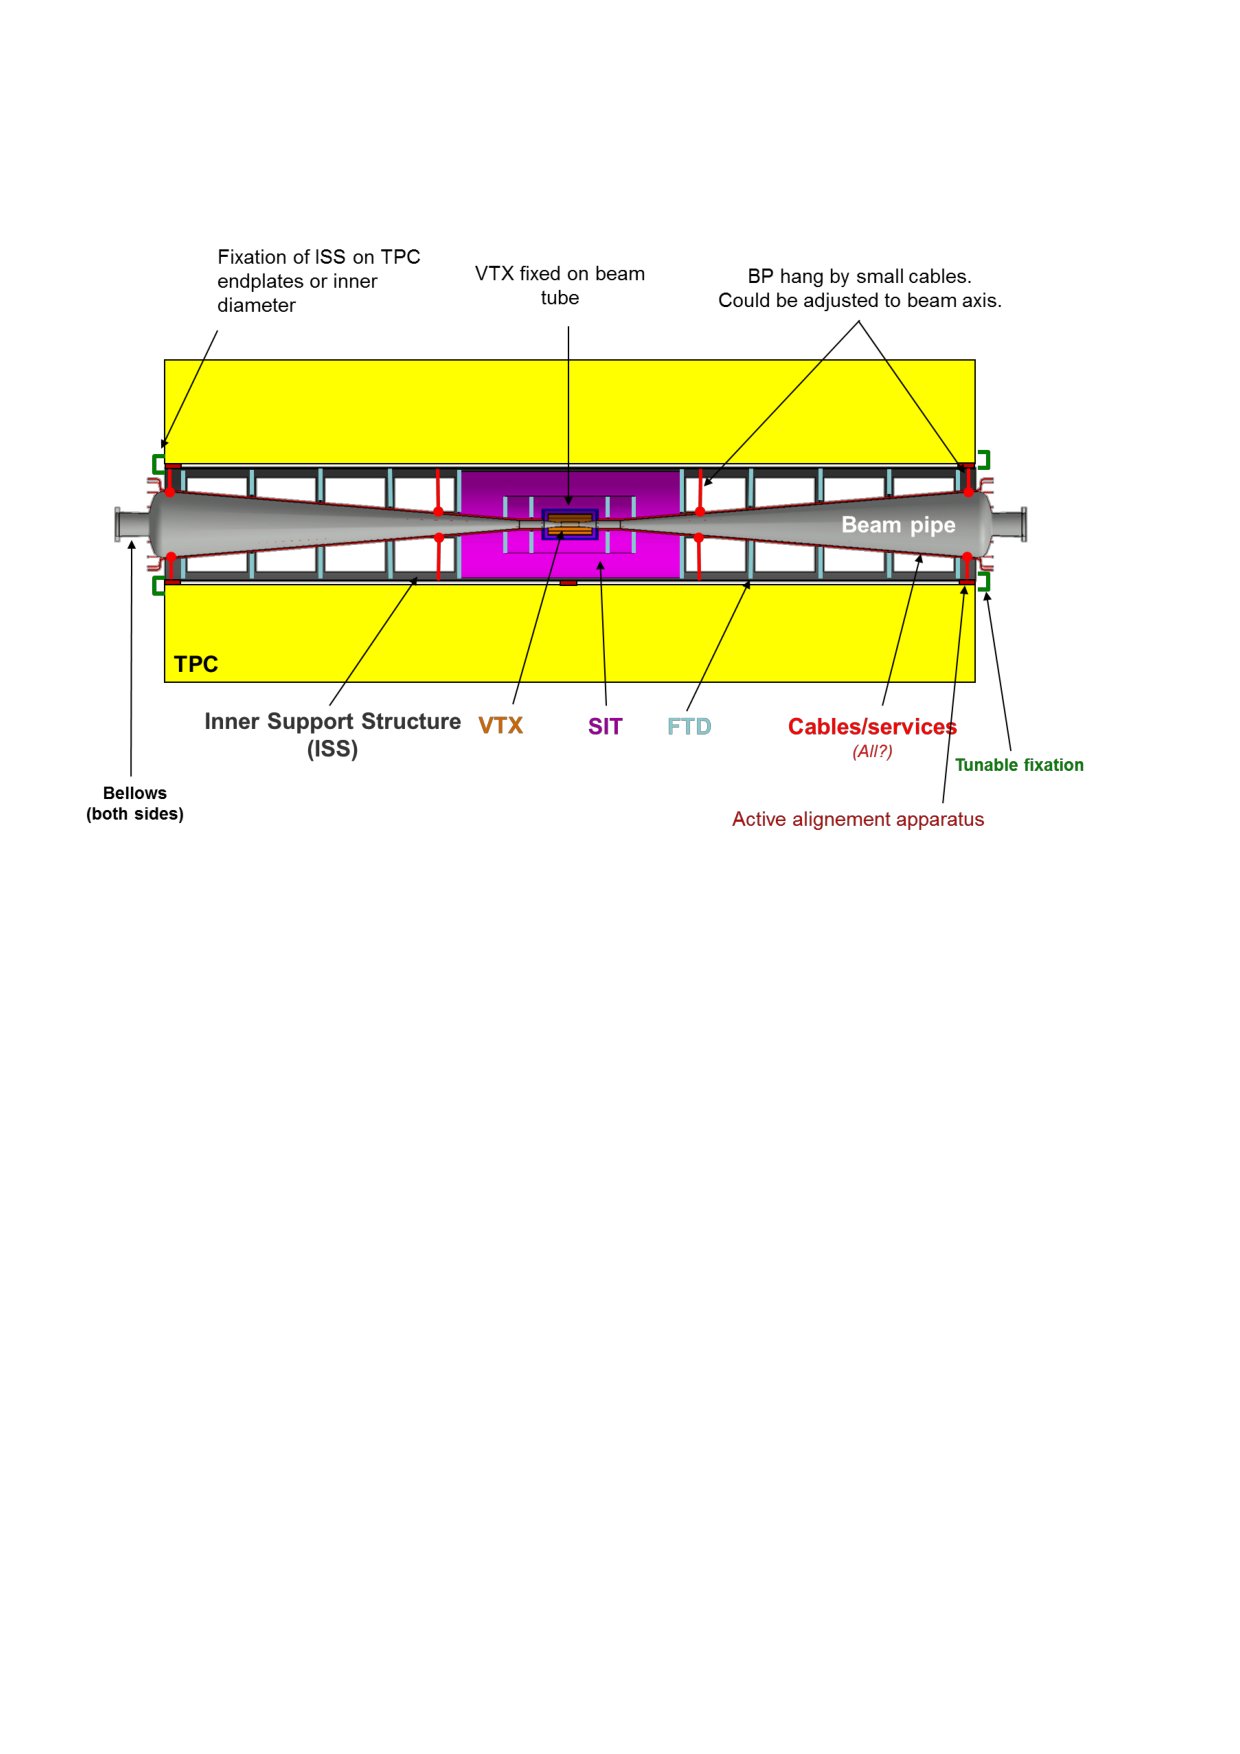
\includegraphics[width=0.8\hsize]{Integration/fig/Inner_Detector_Schematic.pdf}
    \caption{Schematic of the inner tracking detector system~\cite{ild:bib:inner_detector_integration}.}
    \label{ILD:fig:inner_detector_schematic}
\end{figure}

\begin{figure}[h!]
    \centering
        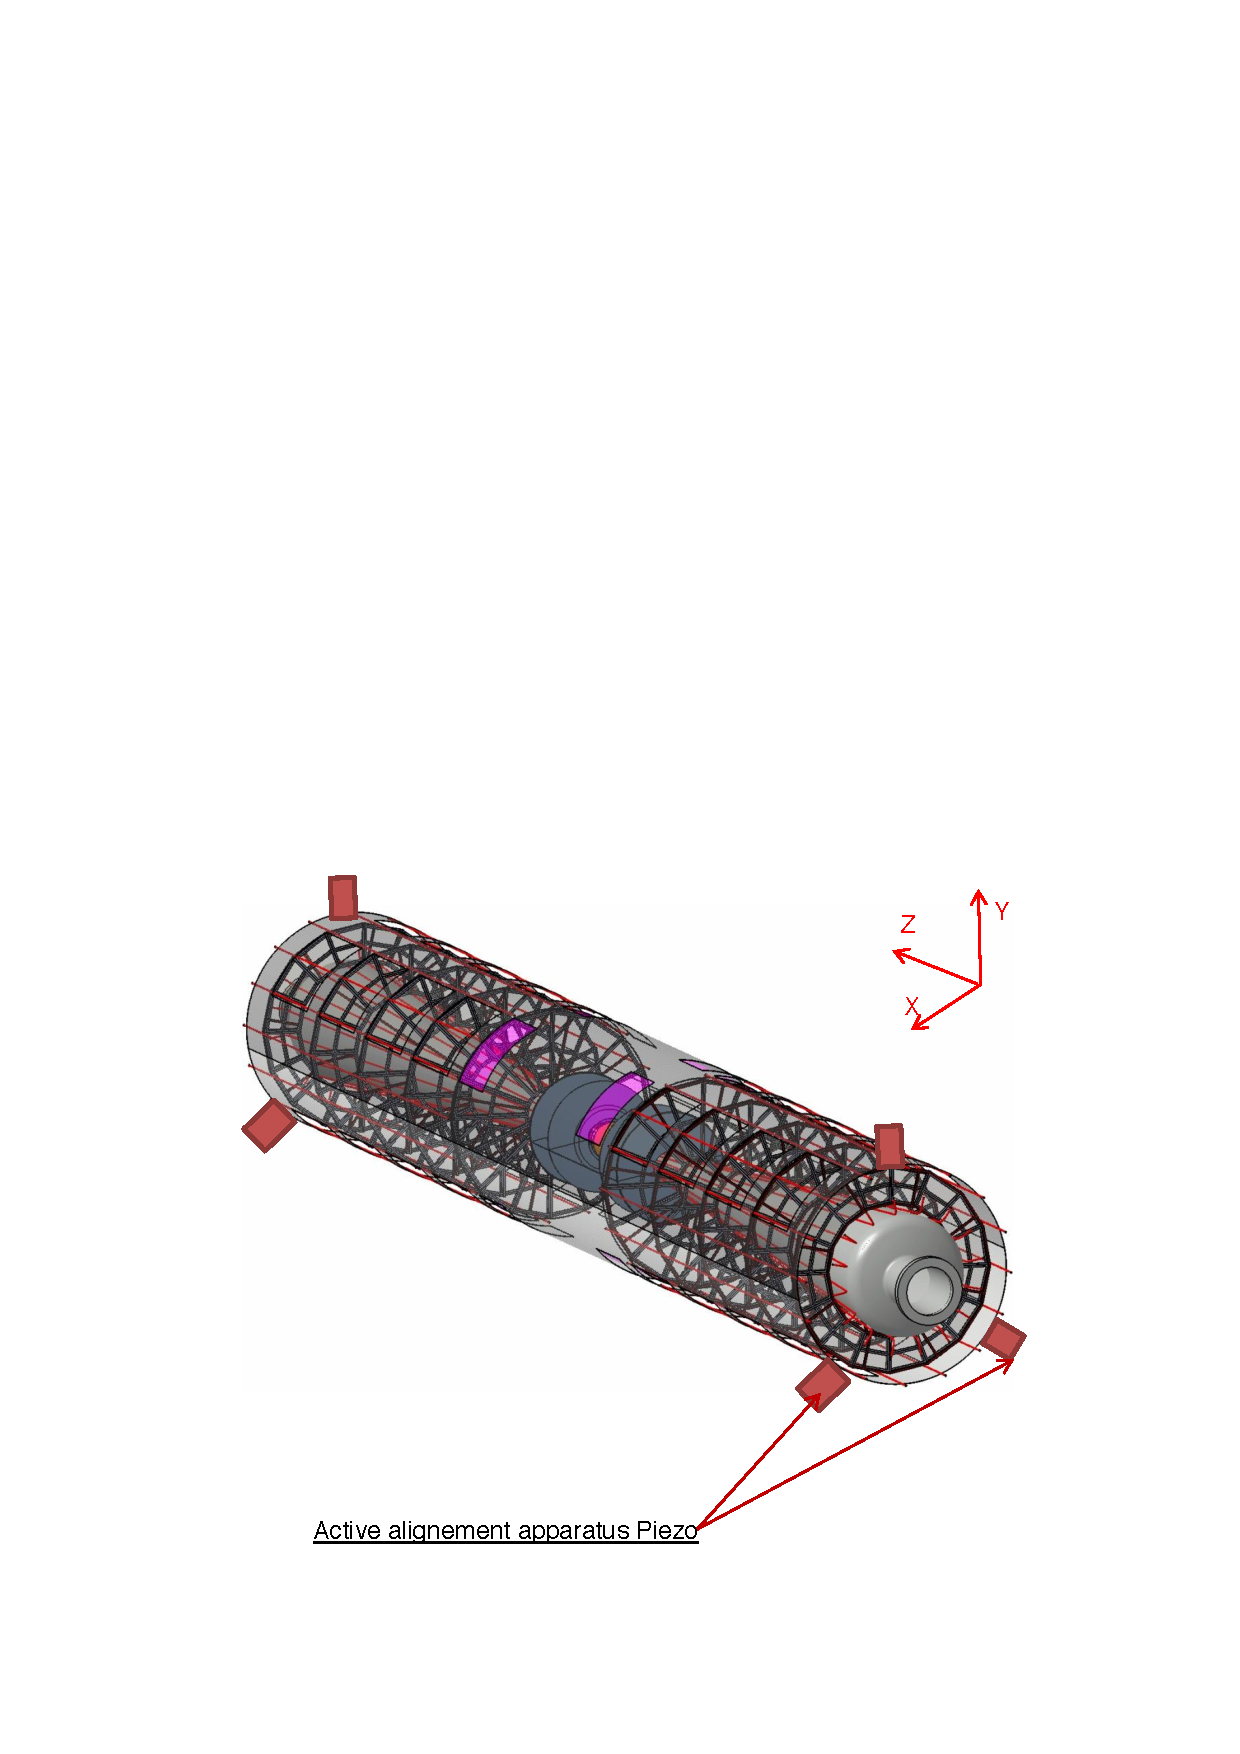
\includegraphics[width=0.8\hsize]{Integration/fig/Inner_Detector_Integration.pdf}
    \caption{Engineering design of the inner detector~\cite{ild:bib:inner_detector_integration}.}
    \label{ILD:fig:inner_detector_integration}
\end{figure}

\subsubsection{Electrical Services and Cooling}
A concept has been developed for the power scheme of the vertex detector (CMOS version), see Figure~\ref{ILD:fig:vtx_services}. Copper based power and control cables as well as optical fibres for the data readout connect the vertex detector with patch panels at either ends of the ISS. From here, the cables are routed as described in section~\ref{ild:sec:services} to the outside of the detector. An engineering design for the details of the cabling and patch panels inside the ISS is still pending. Figure~\ref{ILD:fig:si_services} shows the place holders for the cables in the current model. The vertex detector will be cooled using air flow cooling, where the cooling pipes also need to follow the general services paths.

\begin{figure}[h!]
    \centering
        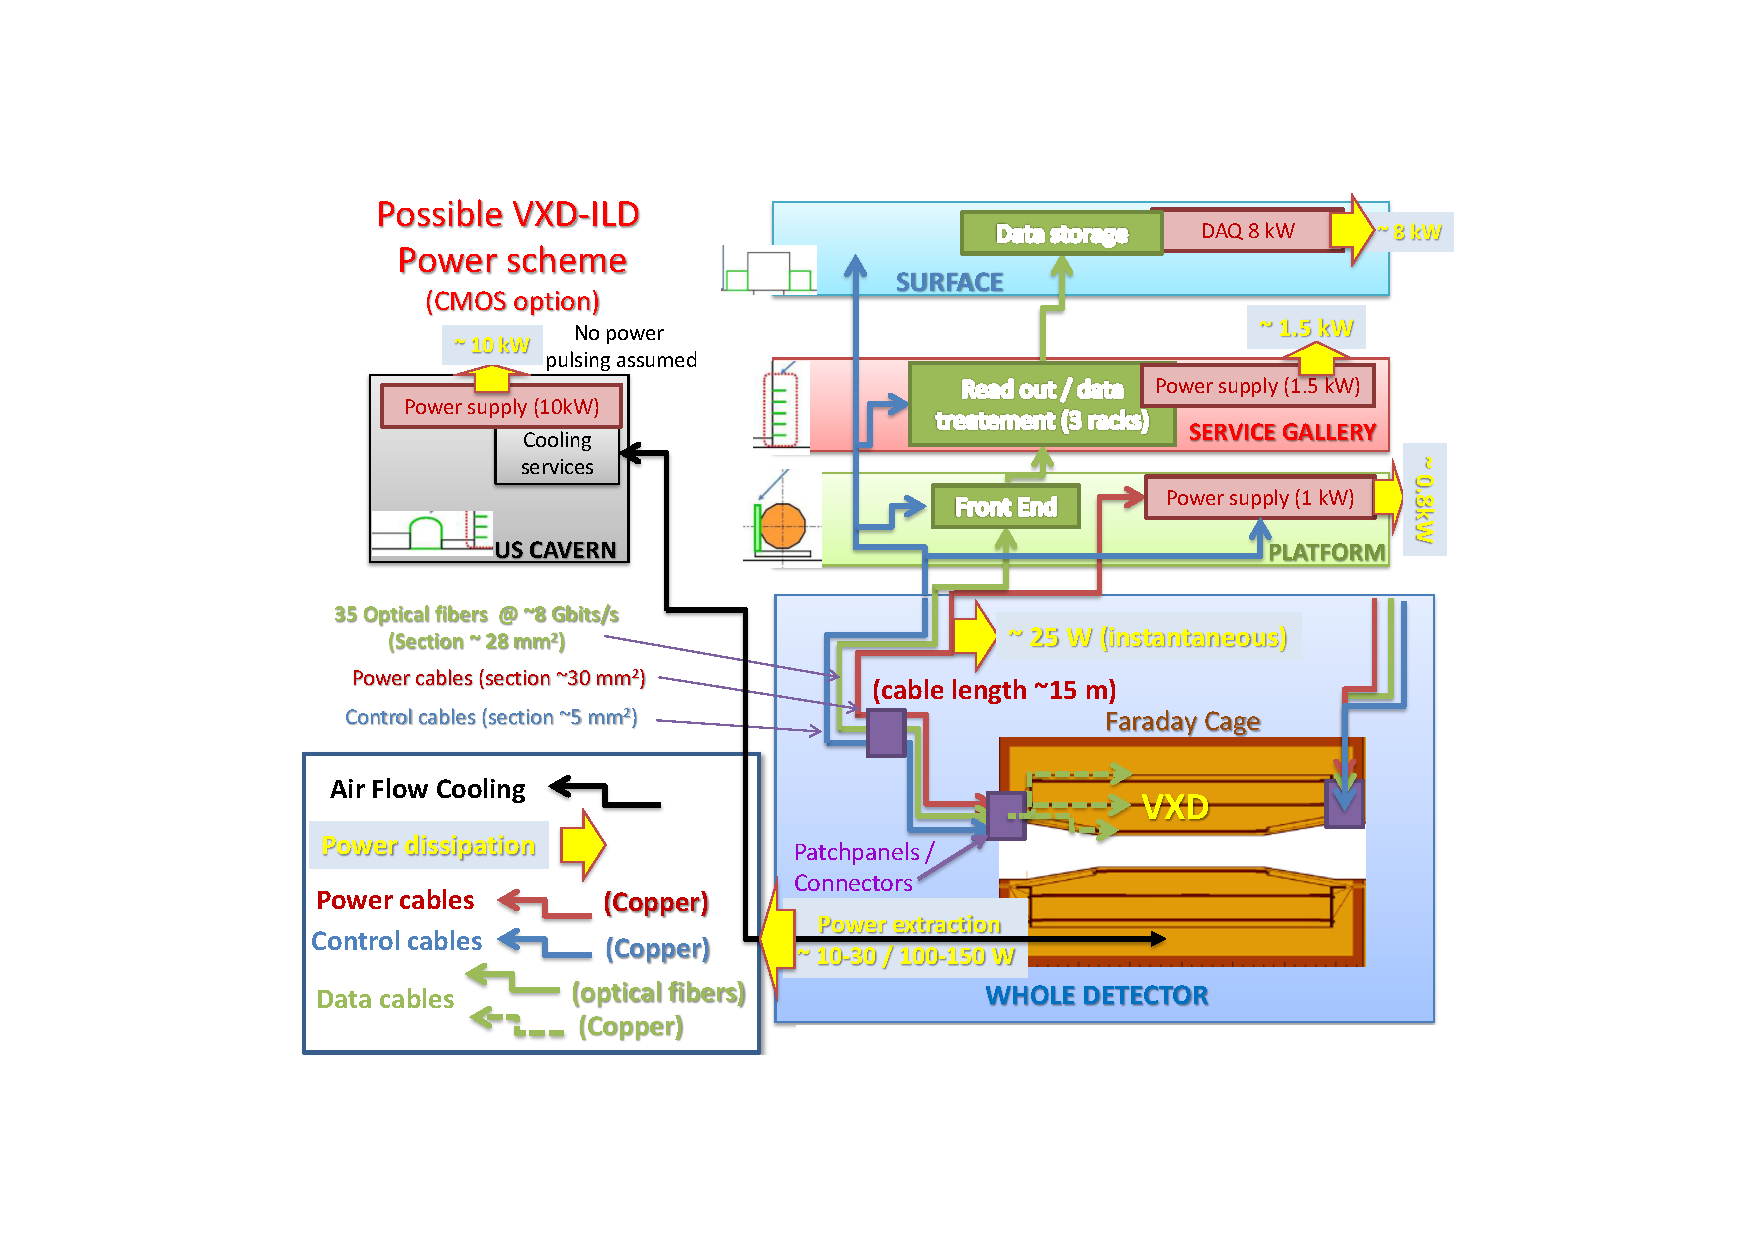
\includegraphics[width=0.8\hsize]{Integration/fig/VTX_services.pdf}
    \caption{Diagram of a power scheme for the vertex detector (CMOS option)~\cite{ild:bib:VTX_integration}.}
    \label{ILD:fig:vtx_services}
\end{figure}

\begin{figure}[h!]
    \centering
        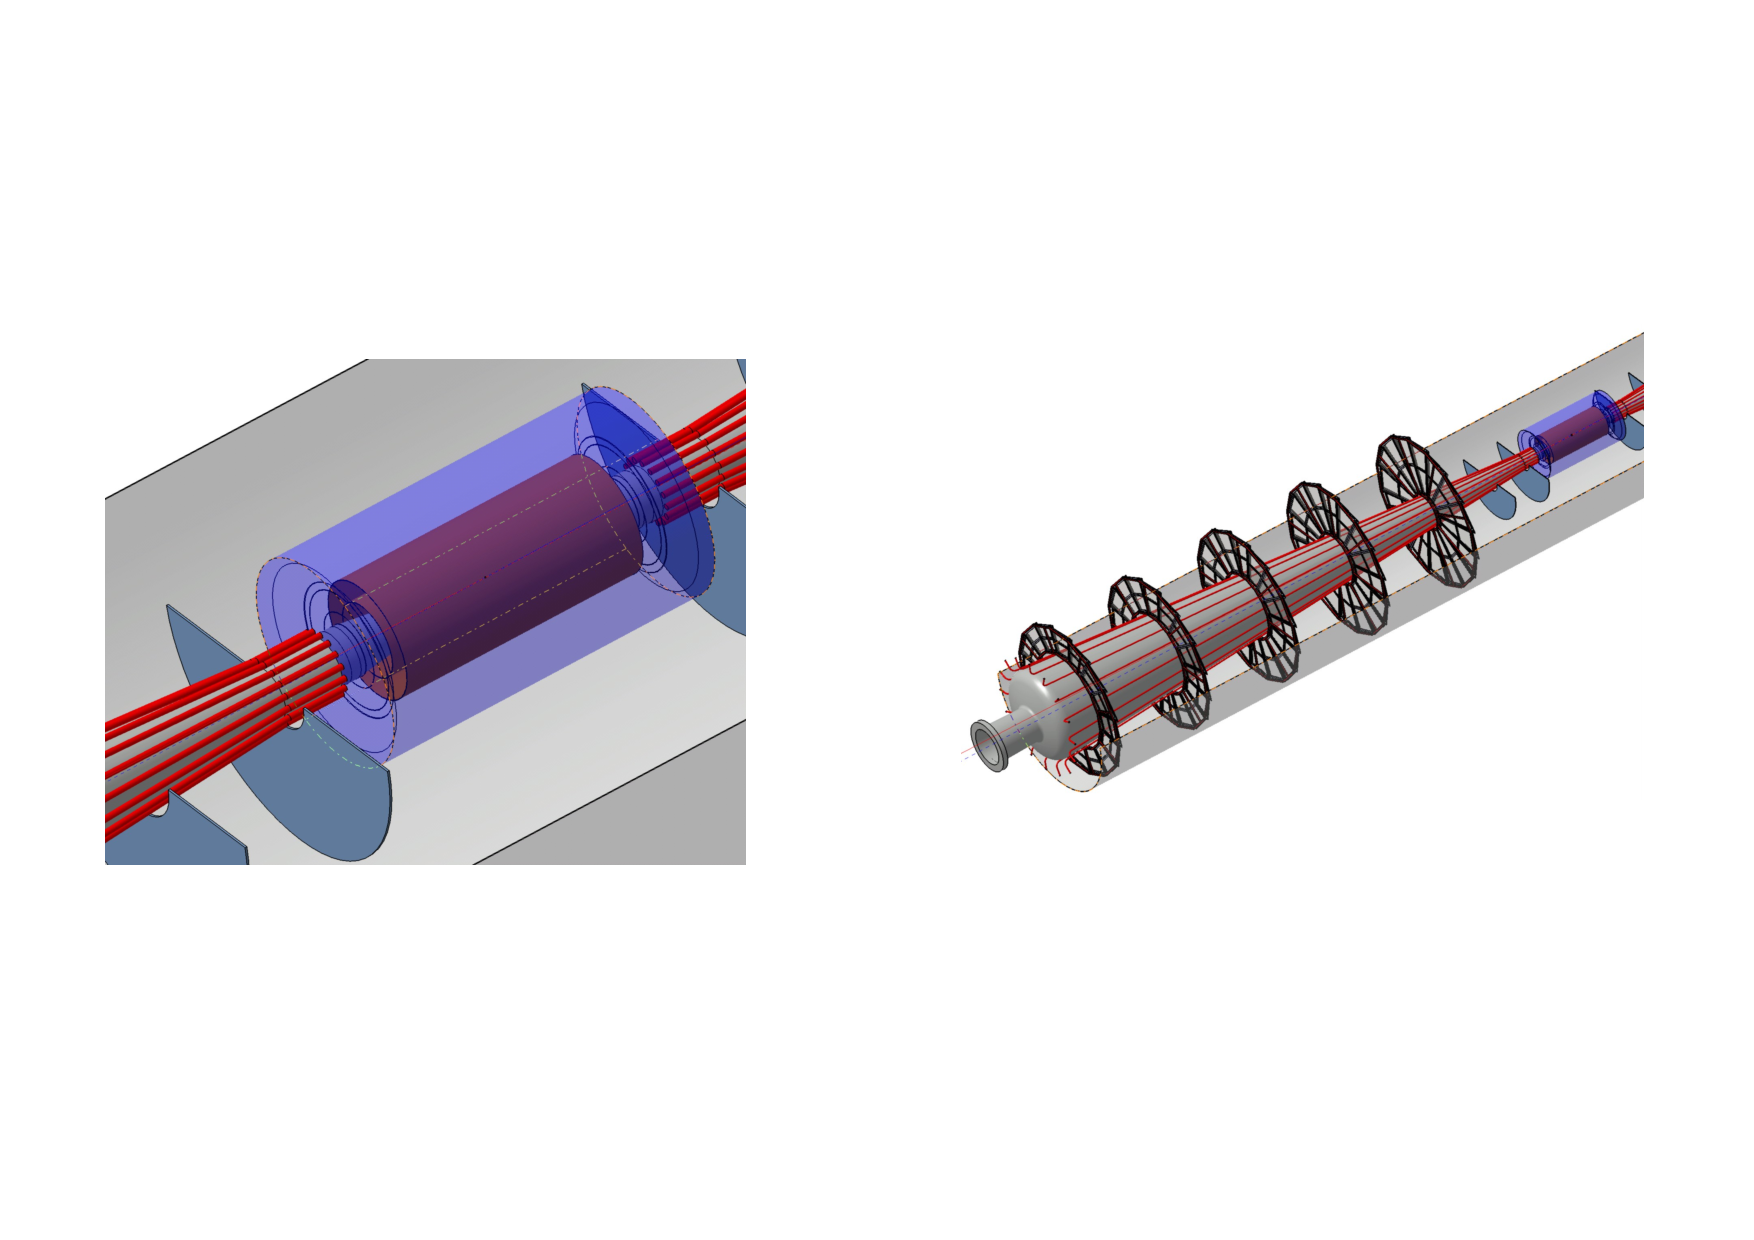
\includegraphics[width=0.8\hsize]{Integration/fig/SI_Services.pdf}
    \caption{Cable placeholders for the inner SI detectors (VTX, SIT, FTD)~\cite{ild:bib:SI_integration}.}
    \label{ILD:fig:si_services}
\end{figure}

\subsection{TPC Integration}

\subsubsection{Mechanical integration}

The mechanical integration of the TPC is still under study. Two possible concepts are being followed up. Either the TPC will be suspended directly from the solenoid cryostat with the help of carbon ribbons or support struts. Or it can be mounted to the absorber structure of the hadronic calorimeter. In the first case, the TPC would be decoupled from the mechanical properties of the calorimeters, at the price of having larger lever arms that might amplify vibrations. A longitudinal damping system would probably be required. In the second case, the lever arms would be much shorter, but the dynamic behaviour of the full system of the cryostat, hadronic and electomagnetic calorimeter as well as the TPC itself needs to be understood. 

\subsubsection{Electrical Services and Cooling}

The electrical services and the cooling pipes of the TPC start on both end plates and will be routed through gaps in the front-faces of the calorimeters, between the end-cap and barrel detectors (c.f.~Figure~\ref{ILD:fig:tpc_cables}). A cooling system based on 2-phase CO2 has been tested in 2014 and 2018 on a system of
7 Micromegas modules. Figure~\ref{ILD:fig:tpc_cooling} shows a solution with a 6-loop geometry. The external supplies of the TPC need to be accommodated in the detector environment: while a gas mixing and supply system will most probably be placed on the surface area, distribution sub-systems need to be closer to the detector, e.g.~on the detector platform. The high-voltage power supplies will be placed in the detector hall at reasonable cable-length distances. Figure~\ref{ILD:fig:tpc_interfaces} shows a schematic drawing of the TPC connections to the outer world.

\begin{figure}[h!]
    \centering
    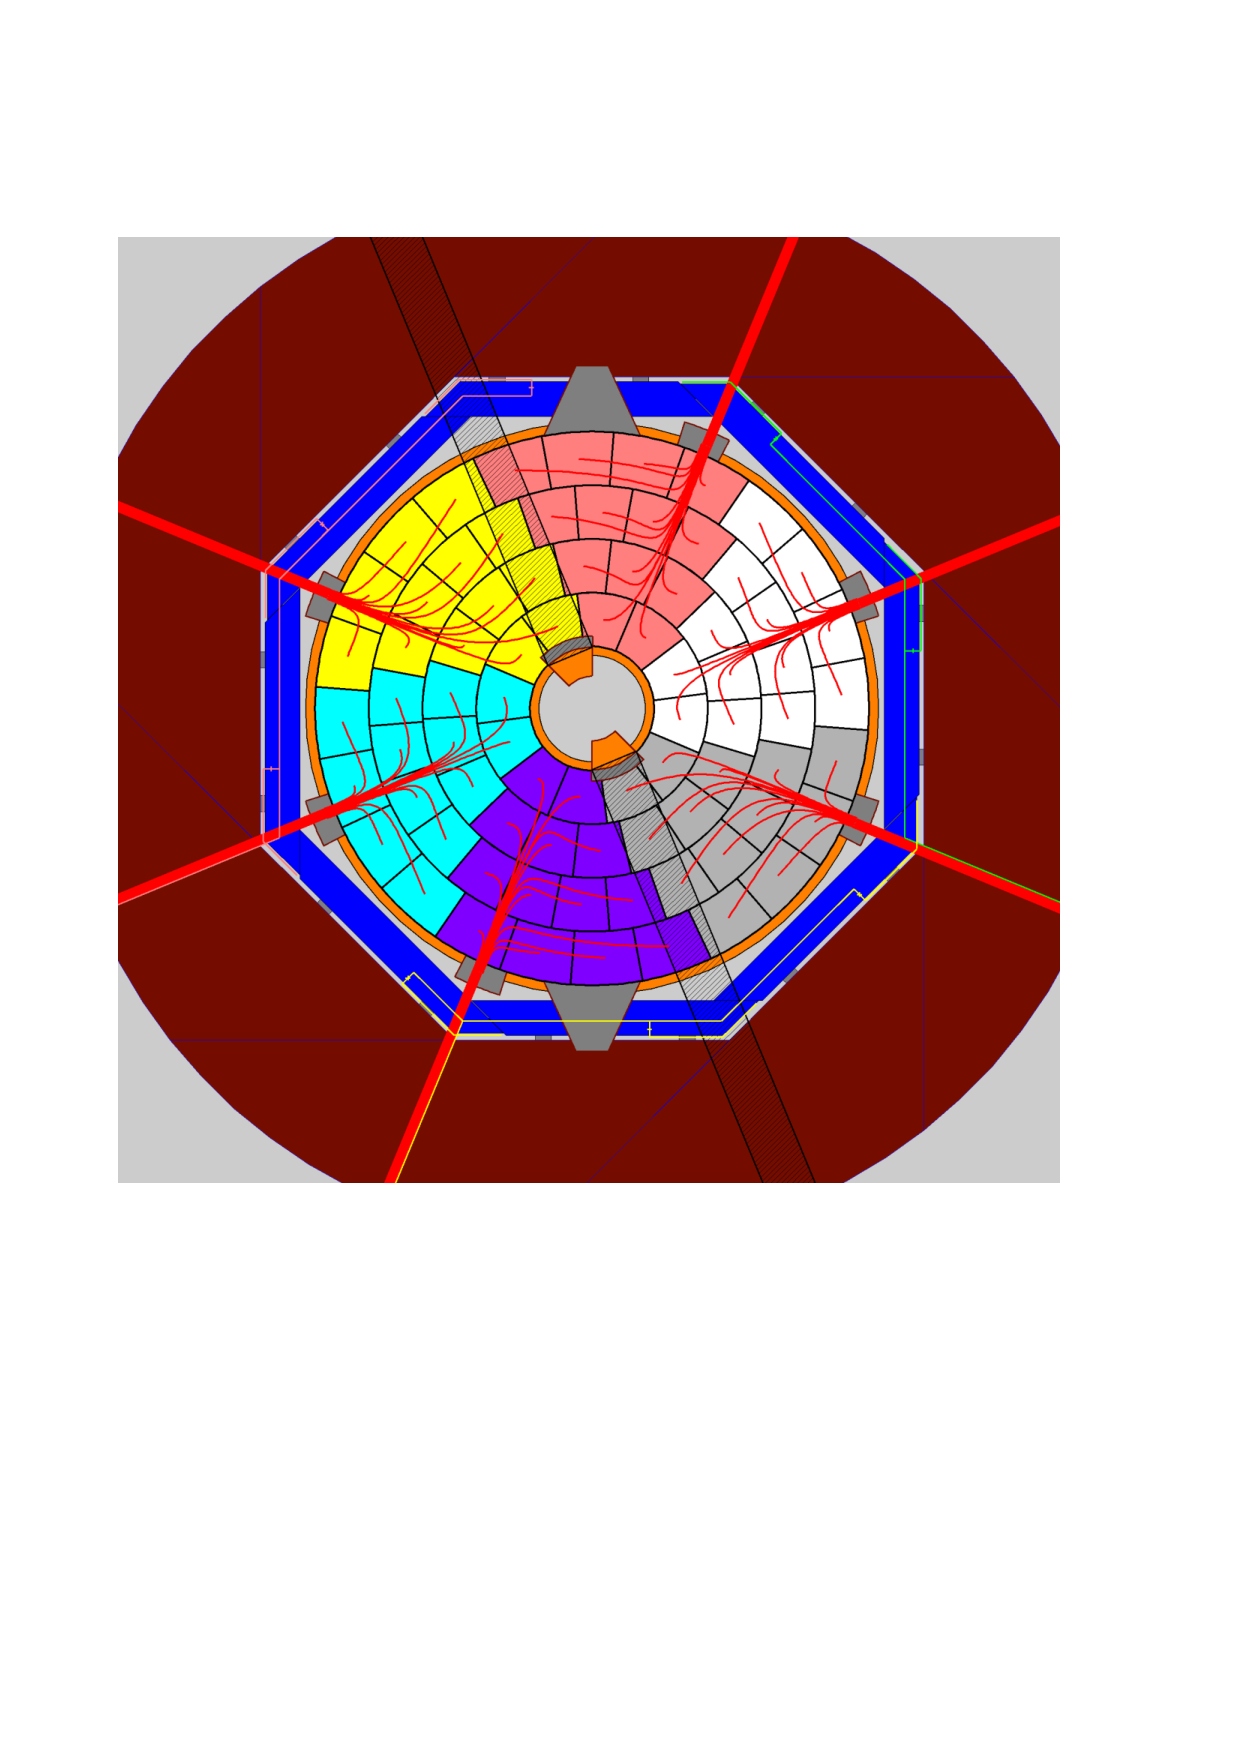
\includegraphics[width=0.6\hsize]{Integration/fig/TPC_Cables.pdf}
    \caption{Sketch of the cable paths on the front-end of the TPC~\cite{ild:bib:TPC_ICD}.}
    \label{ILD:fig:tpc_cables}
\end{figure}
\begin{figure}[h!]
    \centering
    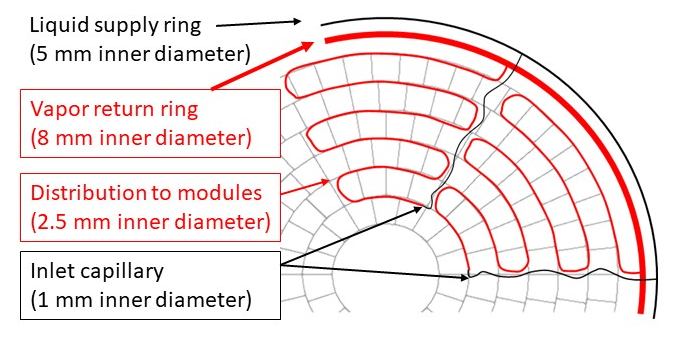
\includegraphics[width=1.0\hsize]{Integration/fig/TPC_Cooling_v2.png}
    \caption{Sketch of a TPC cooling system with tube routing on the TPC end plate. Figure courtesy of Bart Verlaat, Nikhef.}
    \label{ILD:fig:tpc_cooling}
\end{figure}

\begin{figure}[h!]
    \centering
    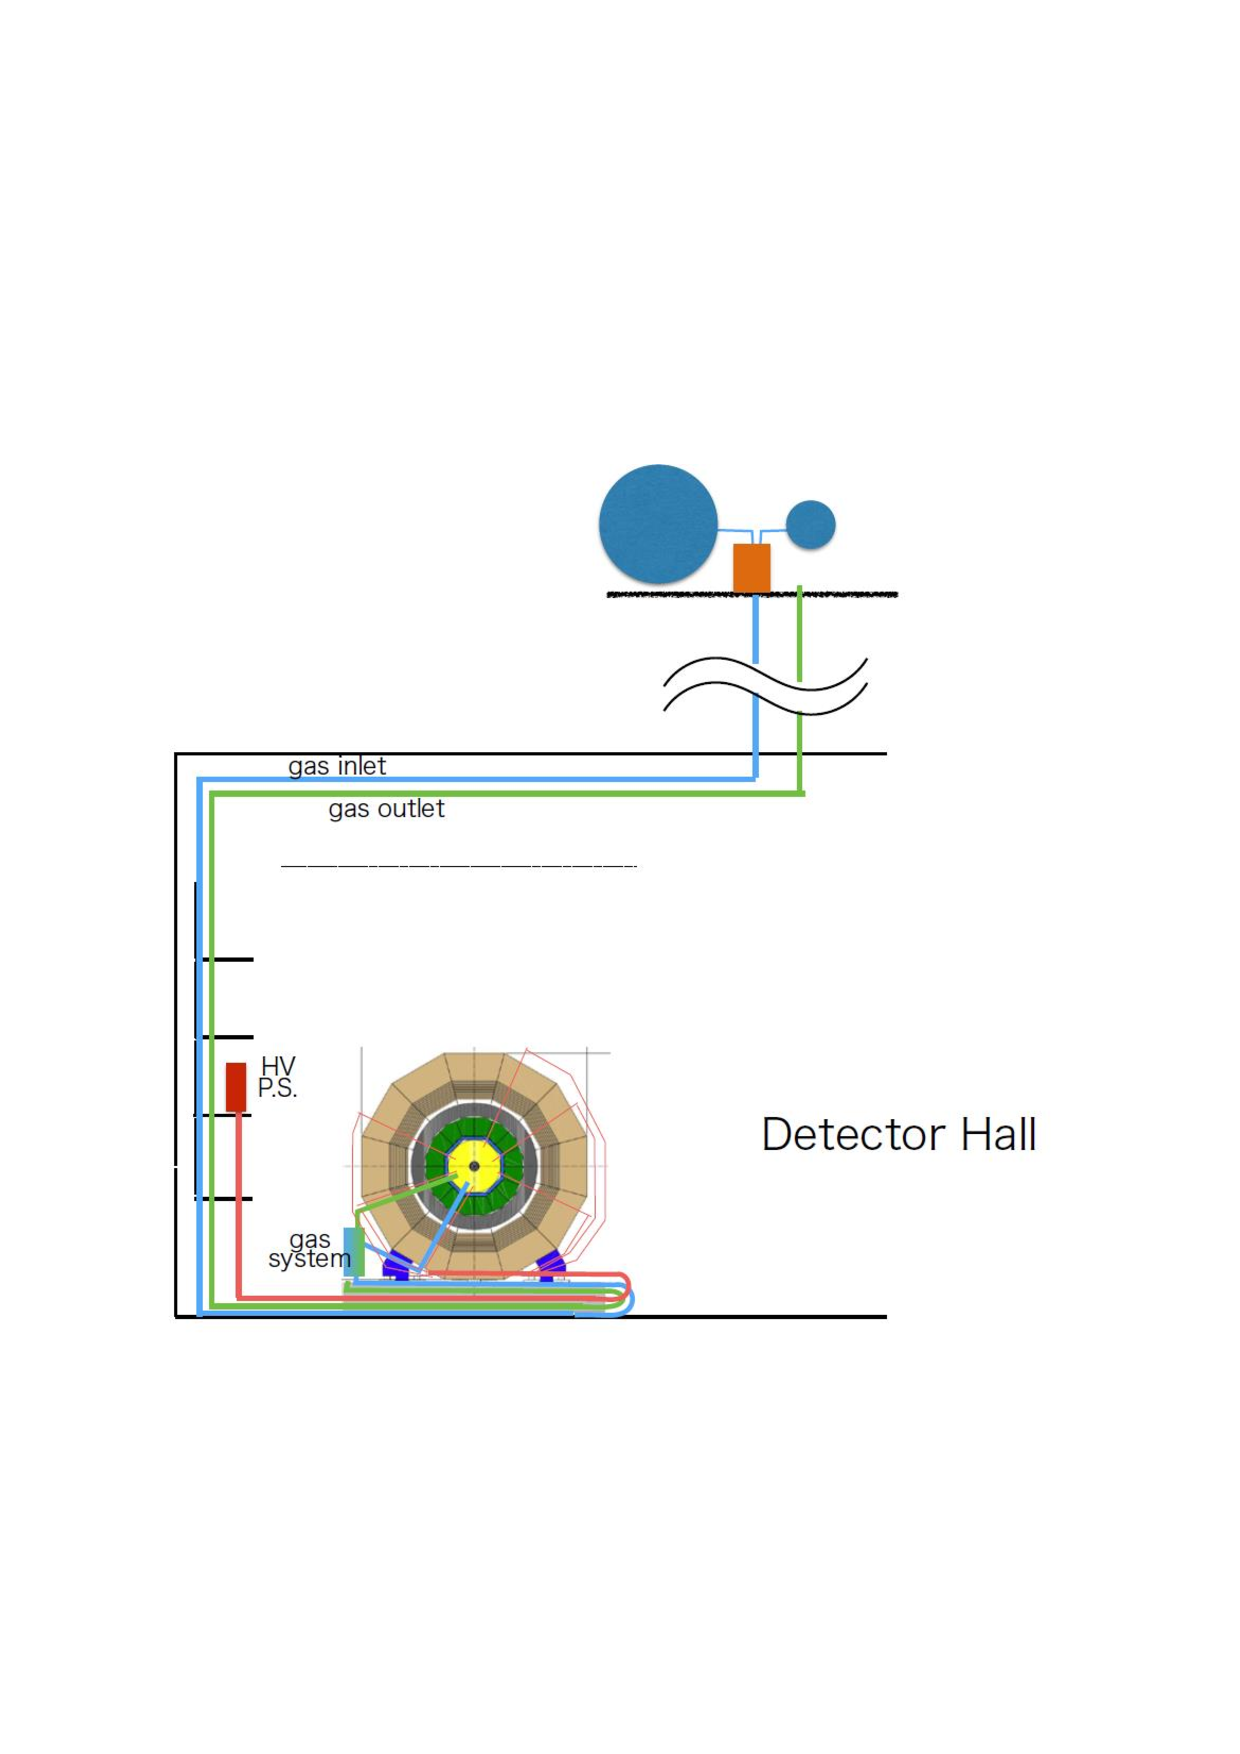
\includegraphics[width=1.0\hsize]{Integration/fig/TPC_Interfaces.pdf}
    \caption{Gas and HV interfaces of the TPC~\cite{ild:bib:TPC_ICD}.}
    \label{ILD:fig:tpc_interfaces}
\end{figure}


\subsection{Electromagnetic Calorimeters Integration}

\subsubsection{Mechanical Integration}

The two options under study for the ILD electromagnetic calorimeters, SiECAL and ScECAL, share the same mechanical design as shown in Figure~\ref{fig:det:ECAL}. The ECAL barrel consists of eight staves that are built from five modules each~(c.f.~figure~\ref{ILD:fig:ECAL_Mechanics}). The staves are supported from the HCAL barrel sections. The ECAL endcaps are supported from the HCAL endcap detector.
\begin{figure}[h]
    \centering
        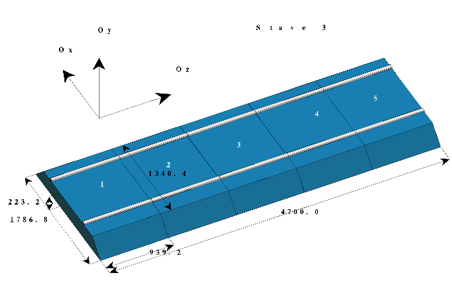
\includegraphics[width=0.5\hsize]{Integration/fig/ECAL_Stave.png}
        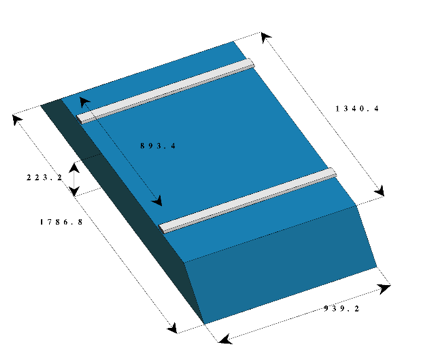
\includegraphics[width=0.3\hsize]{Integration/fig/ECAL_Module.png}
    \caption{ECAL stave and module~\cite{ild:bib:SiECAL_ICD}}
    \label{ILD:fig:ECAL_Mechanics}
\end{figure}

\subsubsection{SiECAL Electrical Services and Cooling}

A detailed integrated design of the SiECAL electrical services and of the cooling system has been developed. Figure~\ref{ILD:fig:siecal_services} shows a close-up view of the upper side of a SiECAL module. The front-end electronics is located at the end of the readout slabs. The services are collected at dedicated hubs for a full column of slabs ("SiECAL Hub2" in the Figure). The service from the column hubs are collected at one central hub for each full stave ("SiECAL Hub1"). Figure~\ref{ILD:fig:siecal_block_diagram} shows a block diagram of the electrical services for the SiECAL and the connections from "Hub1" to the outside power supplies, to the common clock and the DAQ. 

\begin{figure}[h!]
    \centering
        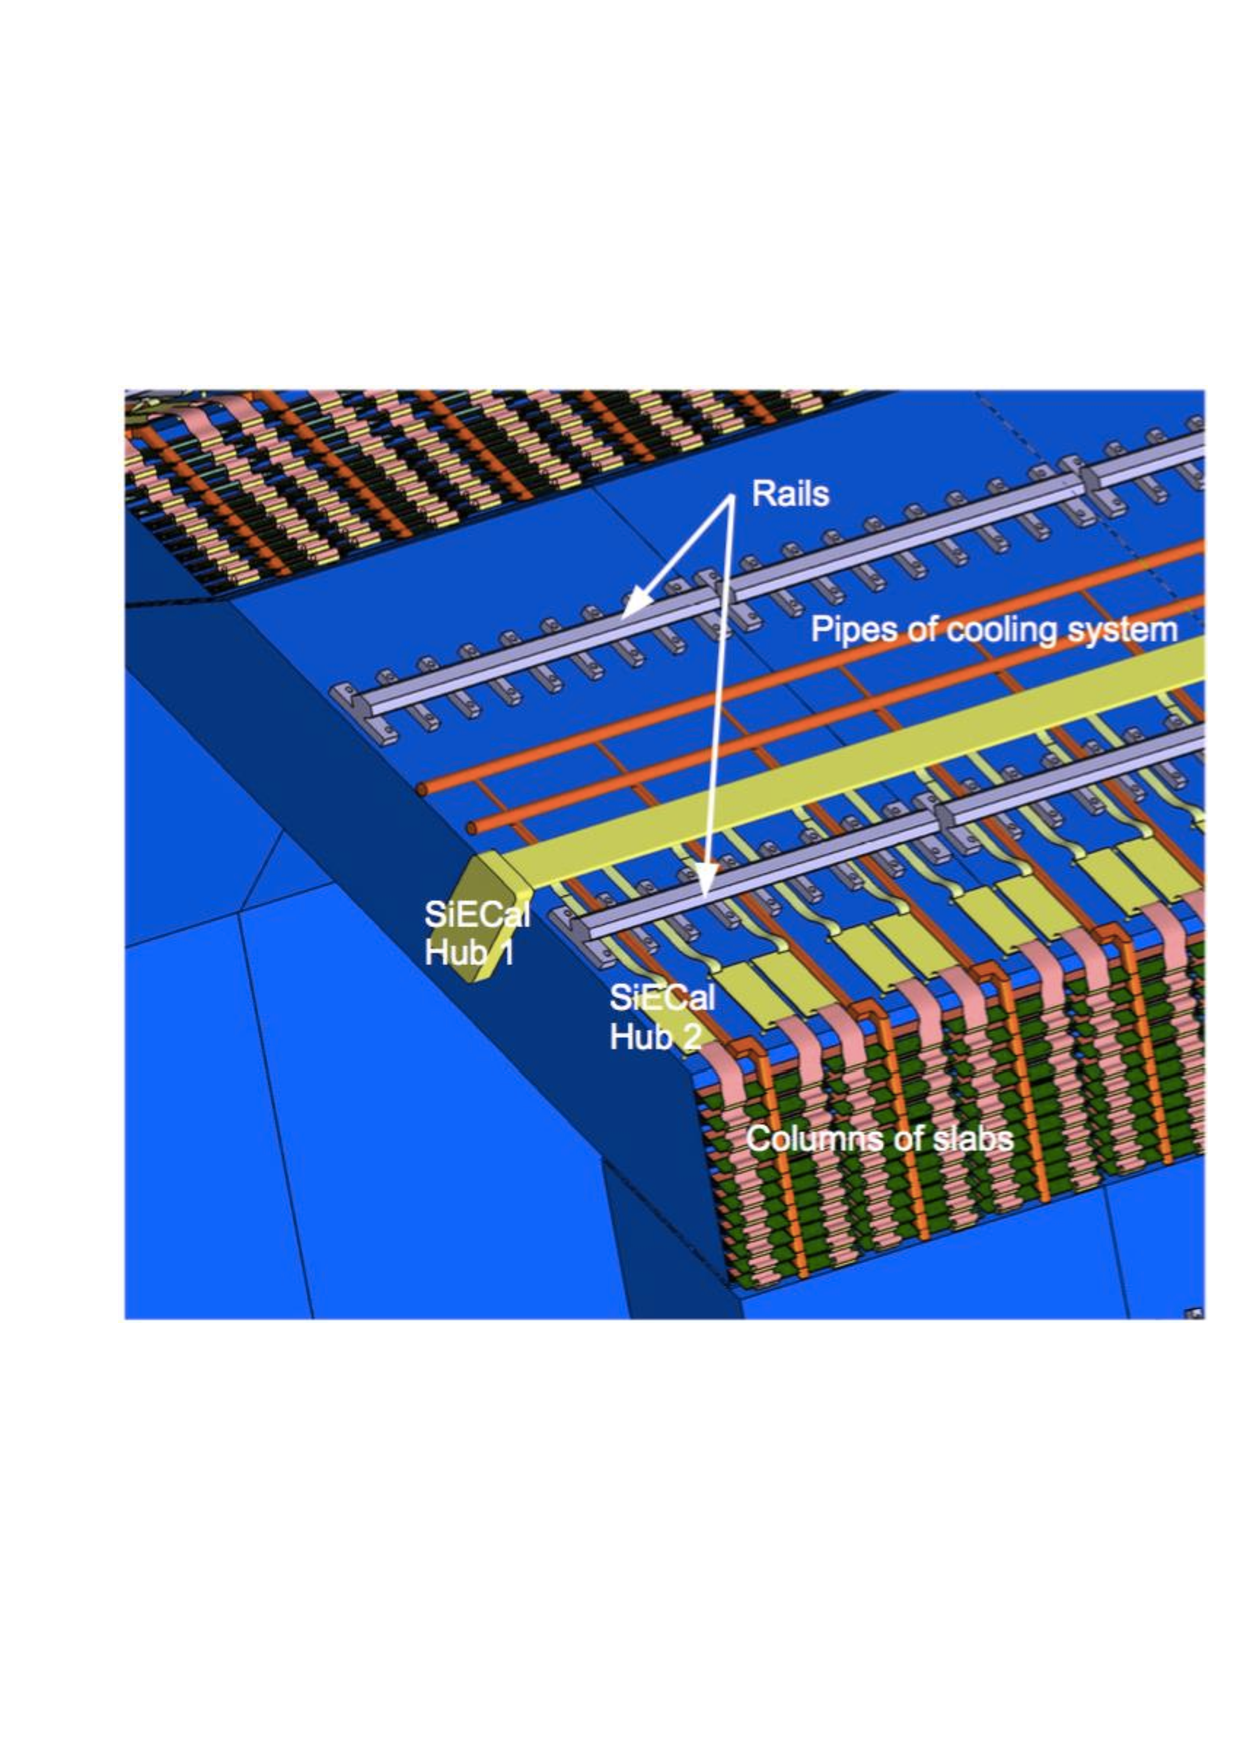
\includegraphics[width=0.6\hsize]{Integration/fig/SiECAL_Services.pdf}
    \caption{Services on an SiECAL module~\cite{ild:bib:SiECAL_ICD}.}
    \label{ILD:fig:siecal_services}
\end{figure}

\begin{figure}[h!]
    \centering
        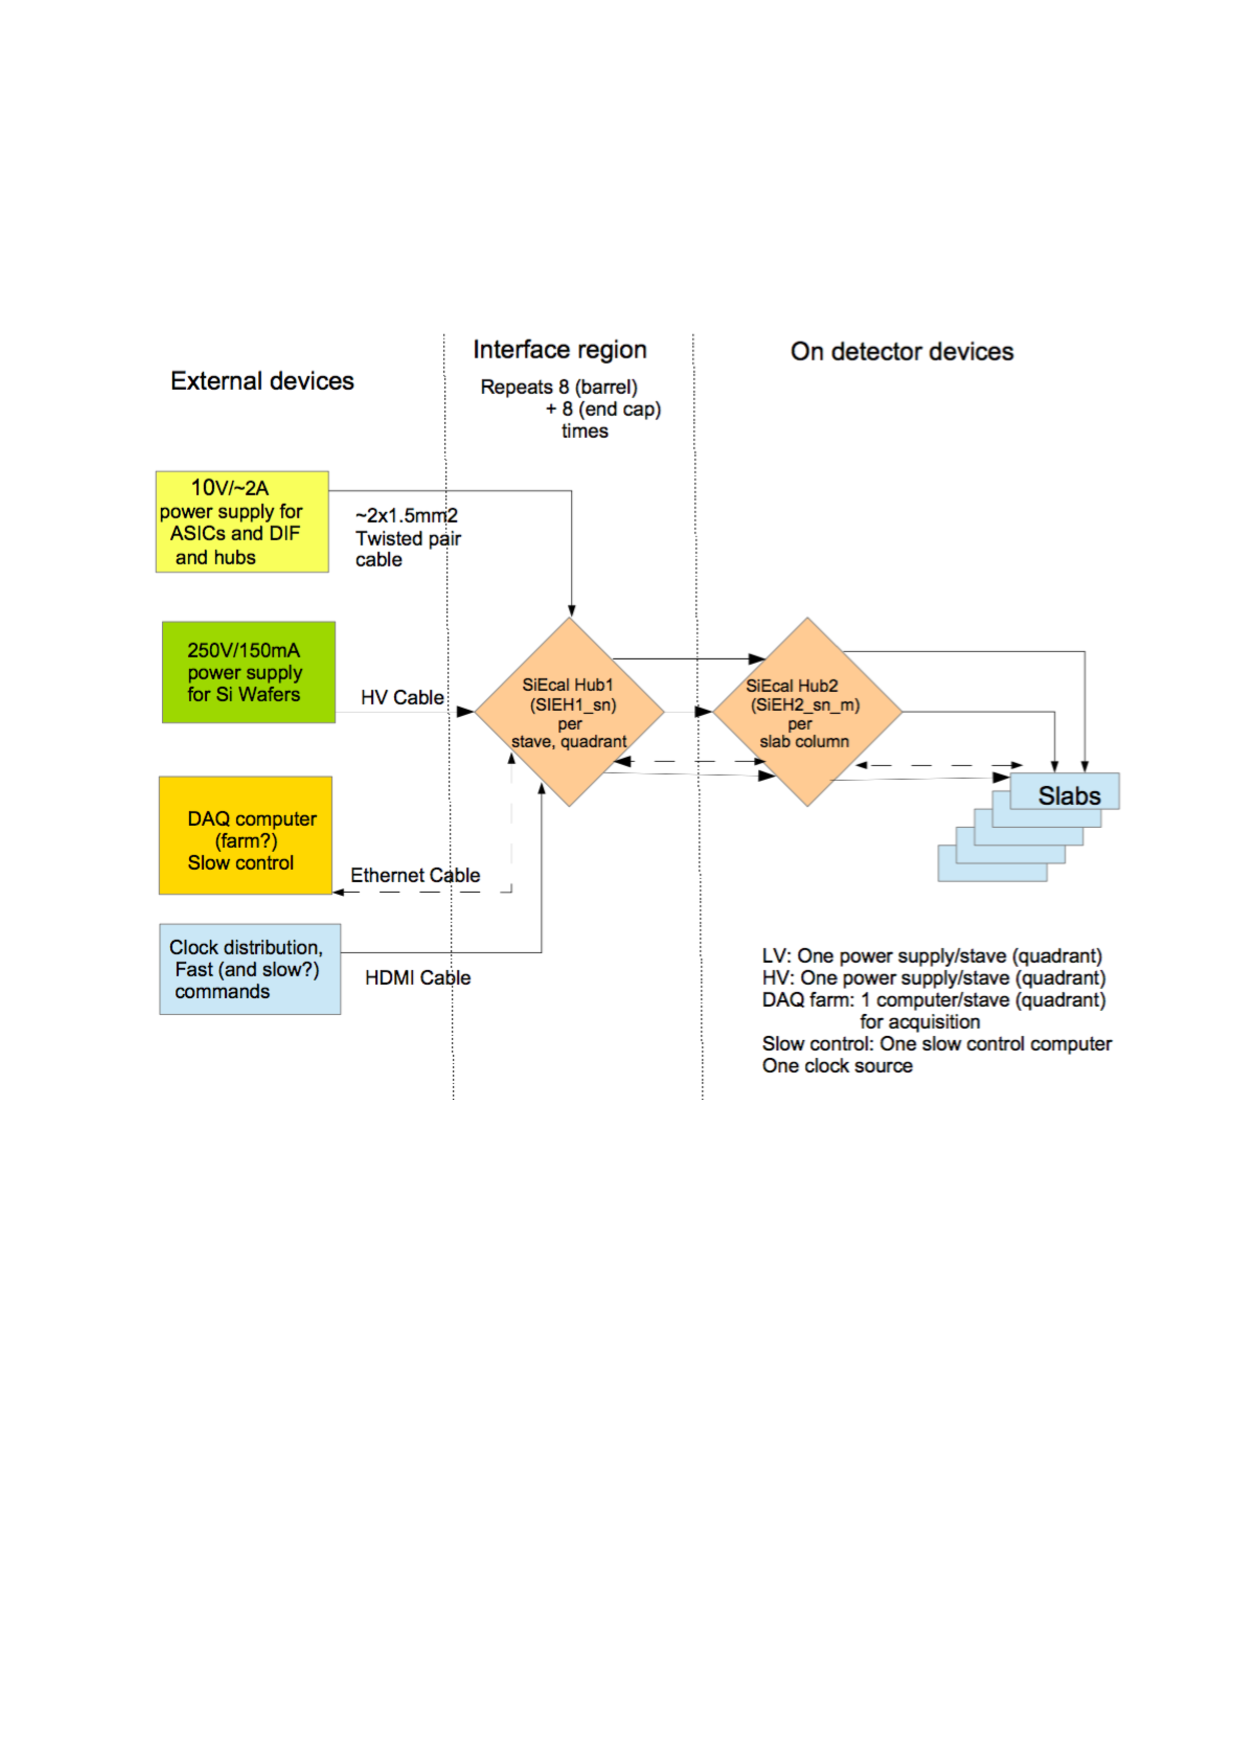
\includegraphics[width=0.8\hsize]{Integration/fig/SiECAL_Block_Diagram.pdf}
    \caption{Block diagram of the electrical services for the SiECAL~\cite{ild:bib:SiECAL_ICD}.}
    \label{ILD:fig:siecal_block_diagram}
\end{figure}

A conceptual design for the SiECAL cooling system is shown in Figure~\ref{ILD:fig:siecal_cooling}. The system foresees leakless water cooling, where a cooling station would be located outside of the ILD detector in the underground area. The water will be distributed via an hierarchical system of cooling lines ("A" to "F") to the barrel and endcap detectors.

\begin{figure}[h!]
    \centering
        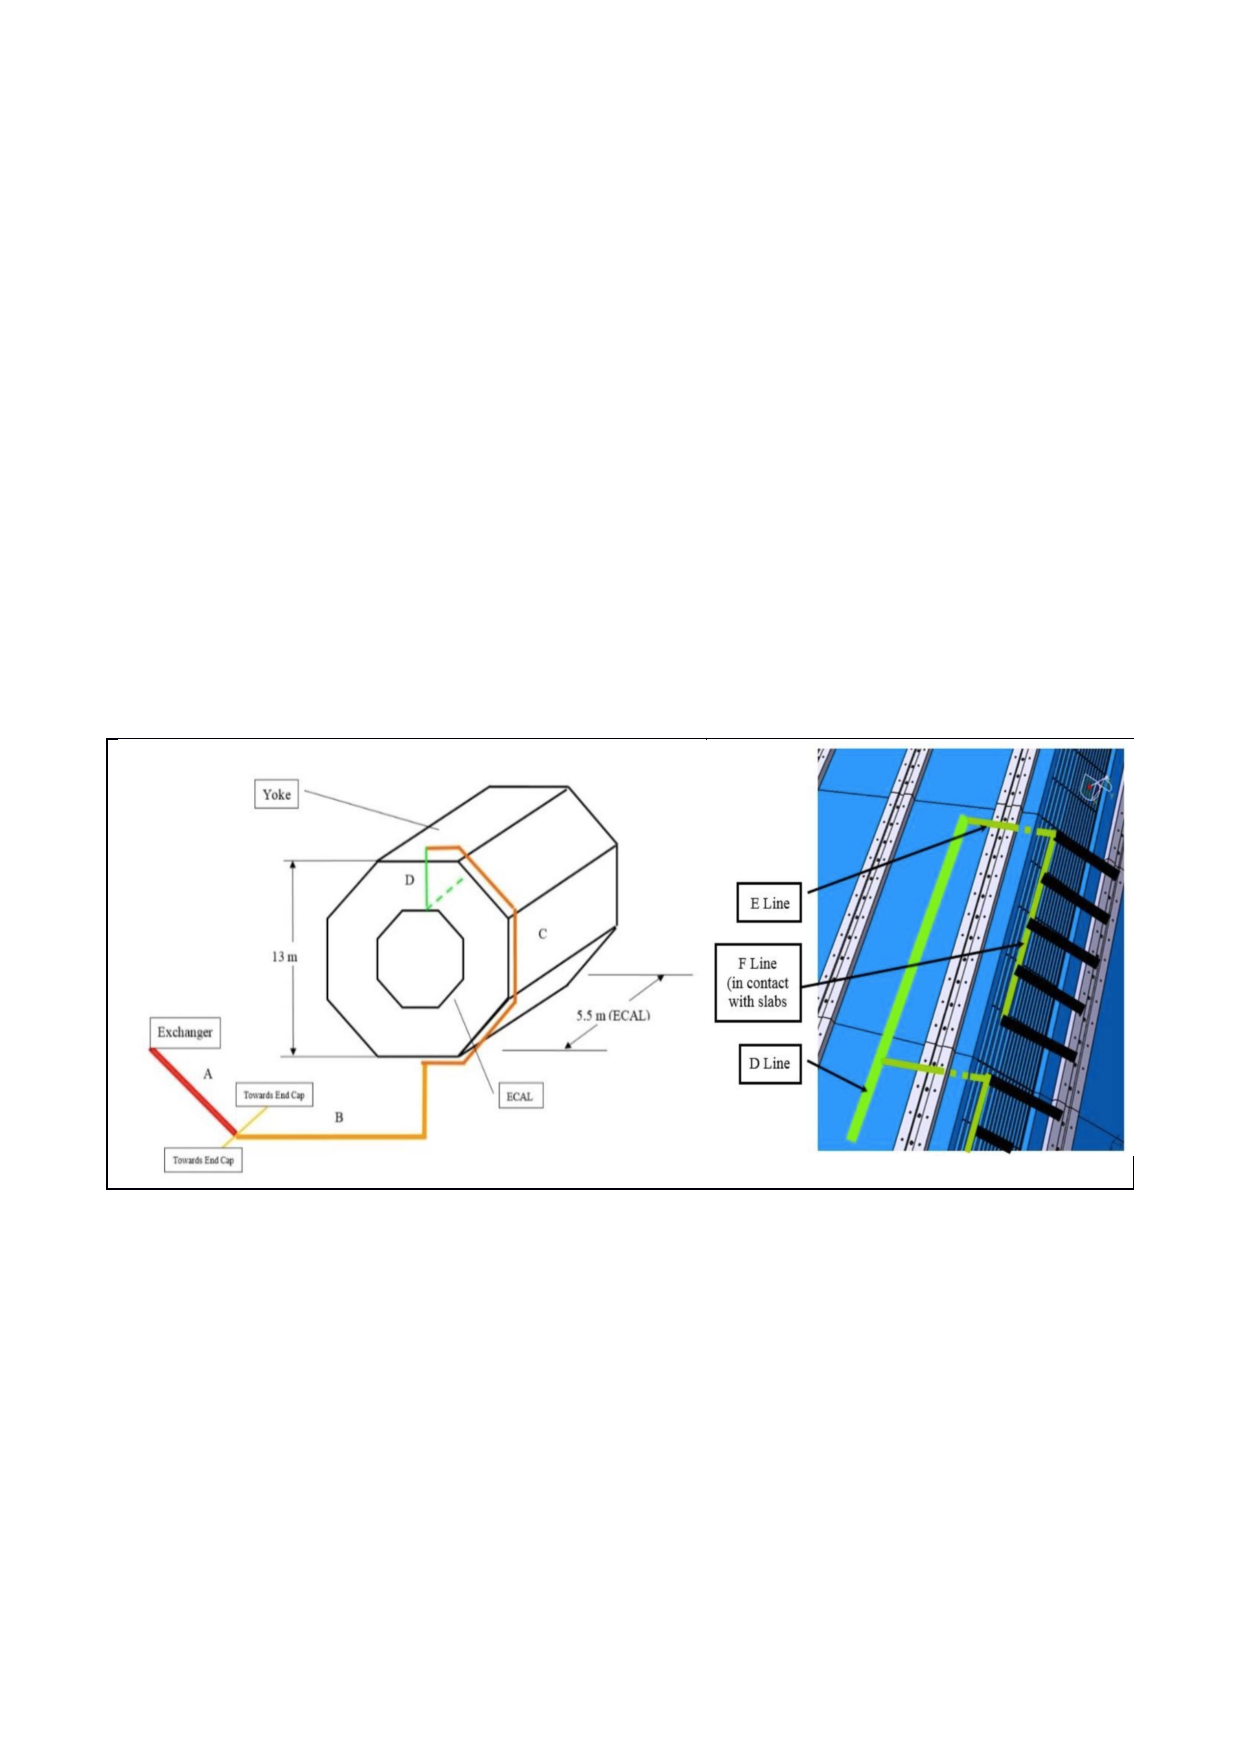
\includegraphics[width=0.8\hsize]{Integration/fig/SiECAL_Cooling.pdf}
    \caption{Conceptual design of the SiECAL cooling system~\cite{ild:bib:SiECAL_ICD}.}
    \label{ILD:fig:siecal_cooling}
\end{figure}

\subsubsection{ScECAL Electrical Services}
The distribution of the electrical services for the ScECAL is very similar to the SiECAL case. Figure~\ref{ILD:fig:scecal_block_diagram} show a block diagram of the service distributions. Also in this case, two series of hubs are planned, one for each stave and one for each column of slabs, to distribute HV and signals accordingly.
\begin{figure}[h!]
    \centering
        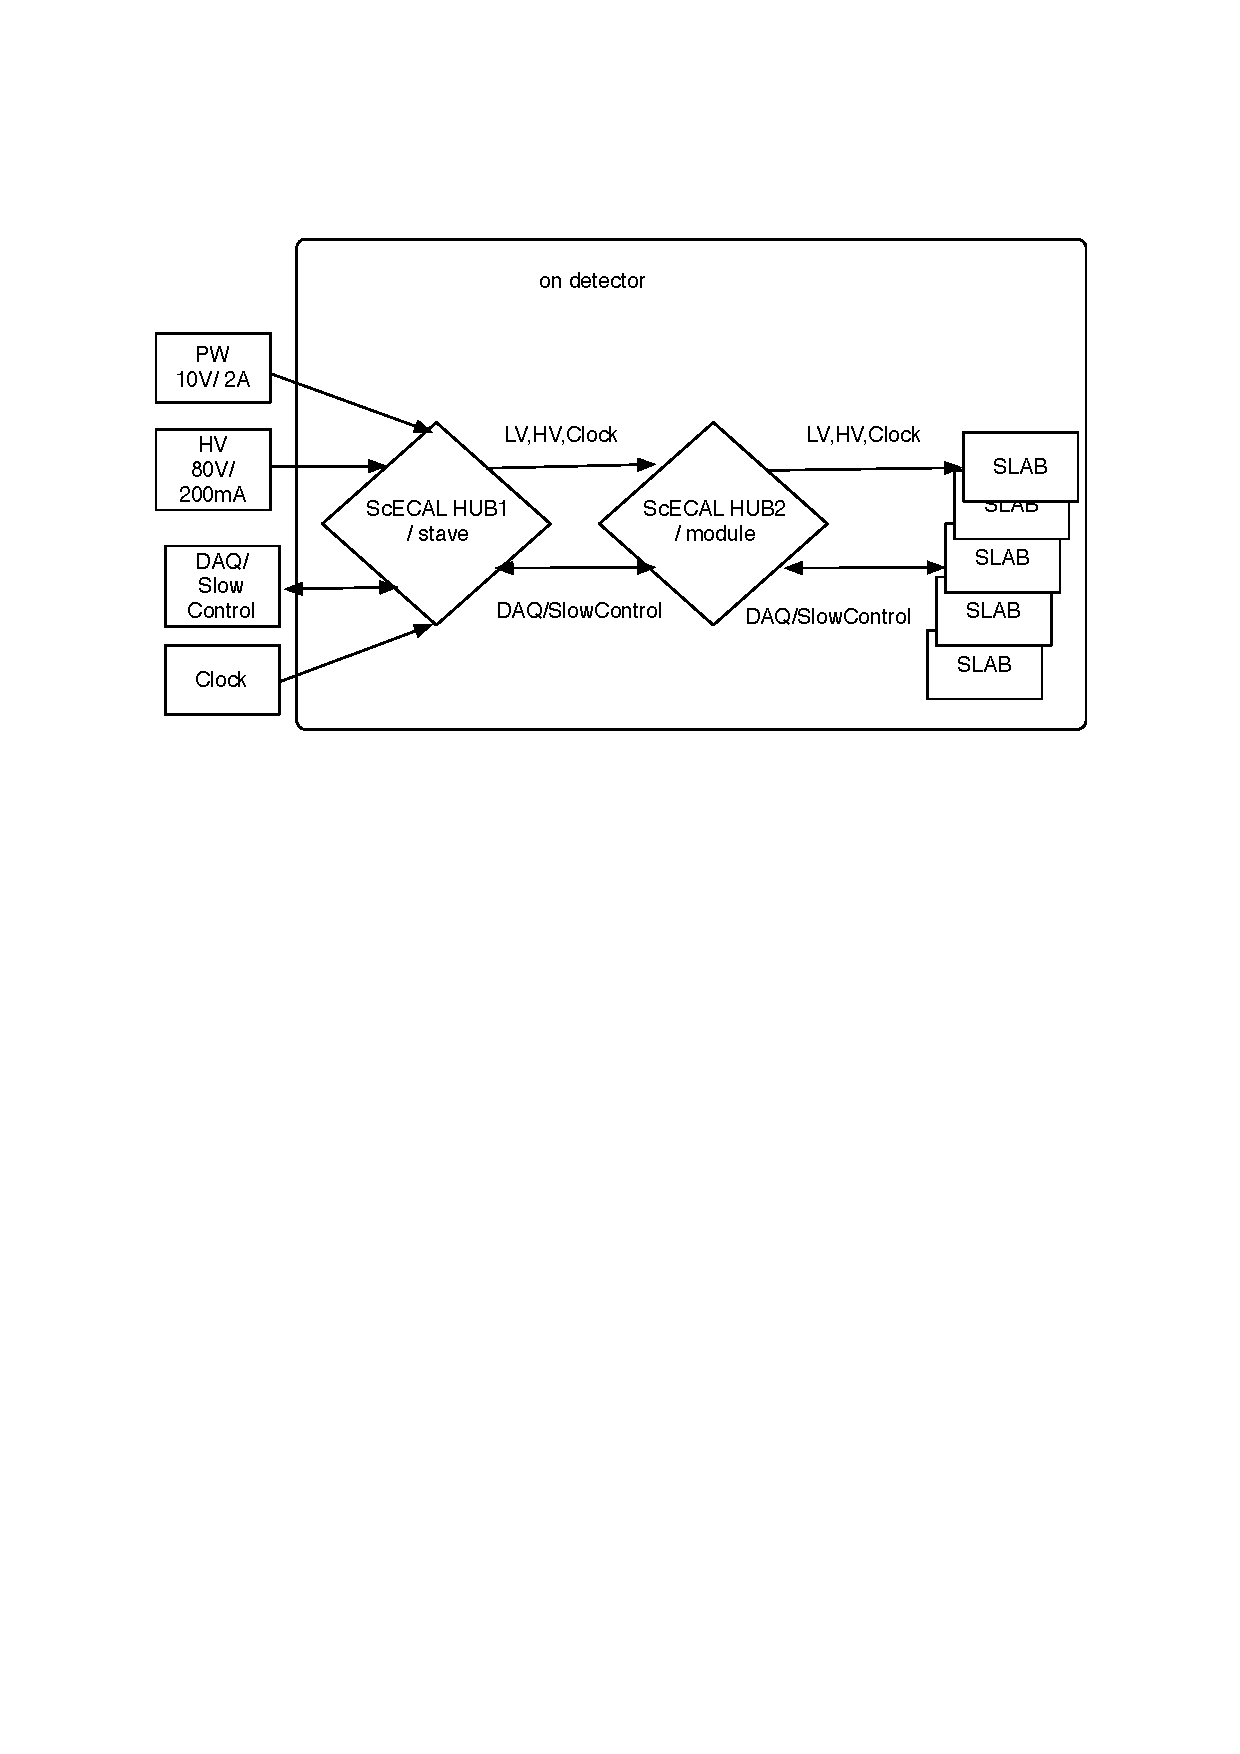
\includegraphics[width=0.8\hsize]{Integration/fig/ScECAL_Block_Diagram.pdf}
    \caption{Block diagram of the electrical services for the ScECAL~\cite{ild:bib:ScECAL_ICD}.}
    \label{ILD:fig:scecal_block_diagram}
\end{figure}


\subsection{Hadronic Calorimeters Integration}
\subsubsection{Mechanical Integration}

Two absorber structures are under study for ILD, the so-called "TESLA" and "Videau" structures~(c.f.~Figure~\ref{fig:det:HCAL}). The main differences from the viewpoint of the detector integration are the mechanical behaviour, further discussed in section~\ref{ild:sec:mechanical_structures}, and the layout of the detector electrical and cooling services. The analogue AHCAL and the semi-digital SDHCAL can be adapted to both mechanical structures. In practice, the AHCAL has been designed with the "TESLA" structure in mind, while the SDHCAL is optimised for the "Videau" case.

\subsubsection{AHCAL Electrical Services and Cooling}
An engineering model of the AHCAL barrel section in the "TESLA" structure has been designed and is shown in Figure~\ref{ILD:fig:ahcal_module_services}. Eight of these modules form a ring, two rings form the barrel detector. The active layers are read out via electronic boards that are located on the outside of the absorber structure. The data concentrators and power interfaces are accessible when the endcaps of the ILD detector are open.  
\begin{figure}[h!]
    \centering
        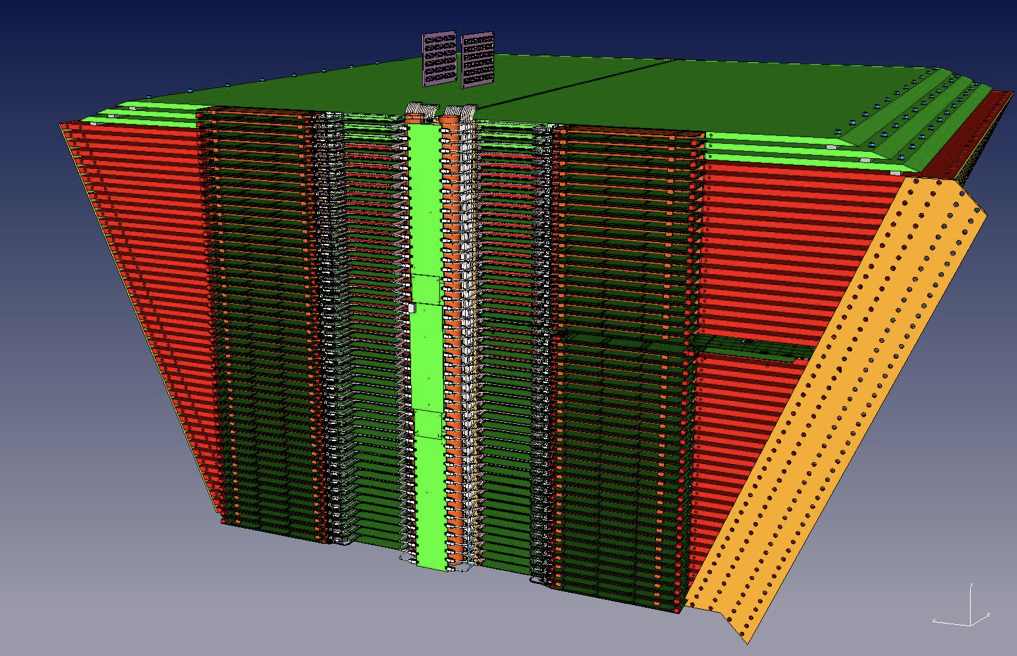
\includegraphics[width=0.8\hsize]{Integration/fig/AHCAL_Module_Services.png}
    \caption{Engineering design of an AHCAL module with electrical and cooling services. Only one instrumented layer is shown for the wedge shape outer parts of the module.1}
    \label{ILD:fig:ahcal_module_services}
\end{figure}
A close-up of the data concentator boards, the electrical services and the cooling system is shown in Figure~\ref{ILD:fig:ahcal_services_closeup}. This service concept has been implemented and successfully used with the AHCAL prototype, Fig.~\ref{fig:AHCAL-TileProto}. The electrical and cooling lines of ECAL, AHCAL, the TPC and the inner detector are routed via the gaps in the AHCAL front between the barrel and the endcap detector, as shown in Figure~\ref{ILD:fig:barrel_services}. 
\begin{figure}[h!]
    \centering
        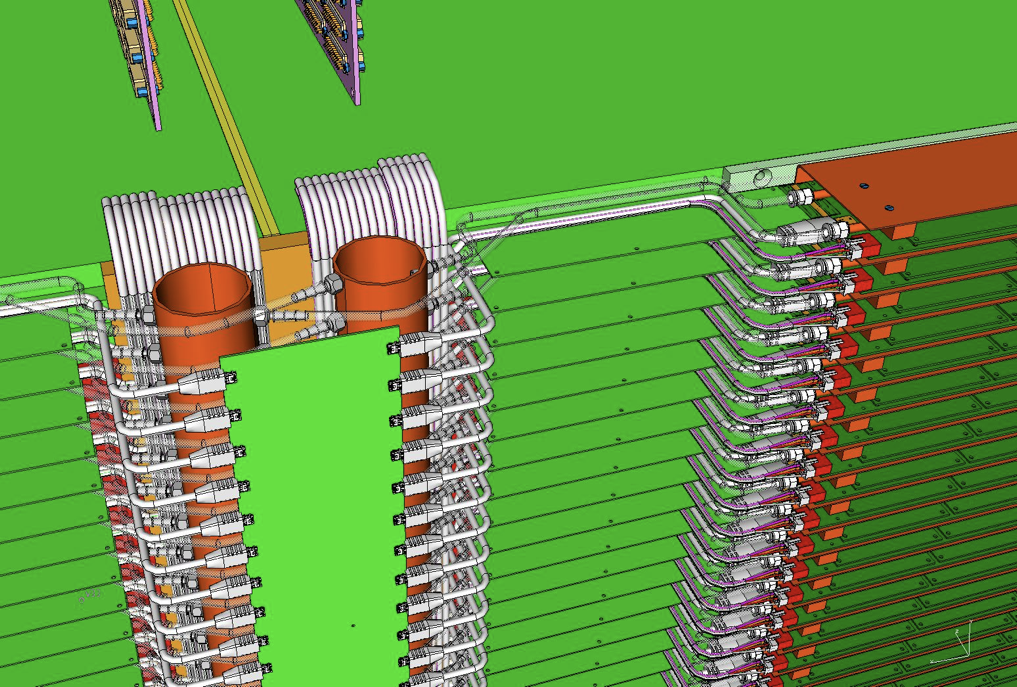
\includegraphics[width=0.9\hsize]{Integration/fig/AHCAL_Services_Closeup.png}
    \caption{AHCAL module front face with readout boards, cables and cooling lines.}
    \label{ILD:fig:ahcal_services_closeup}
\end{figure}
\begin{figure}[h!]
    \centering
        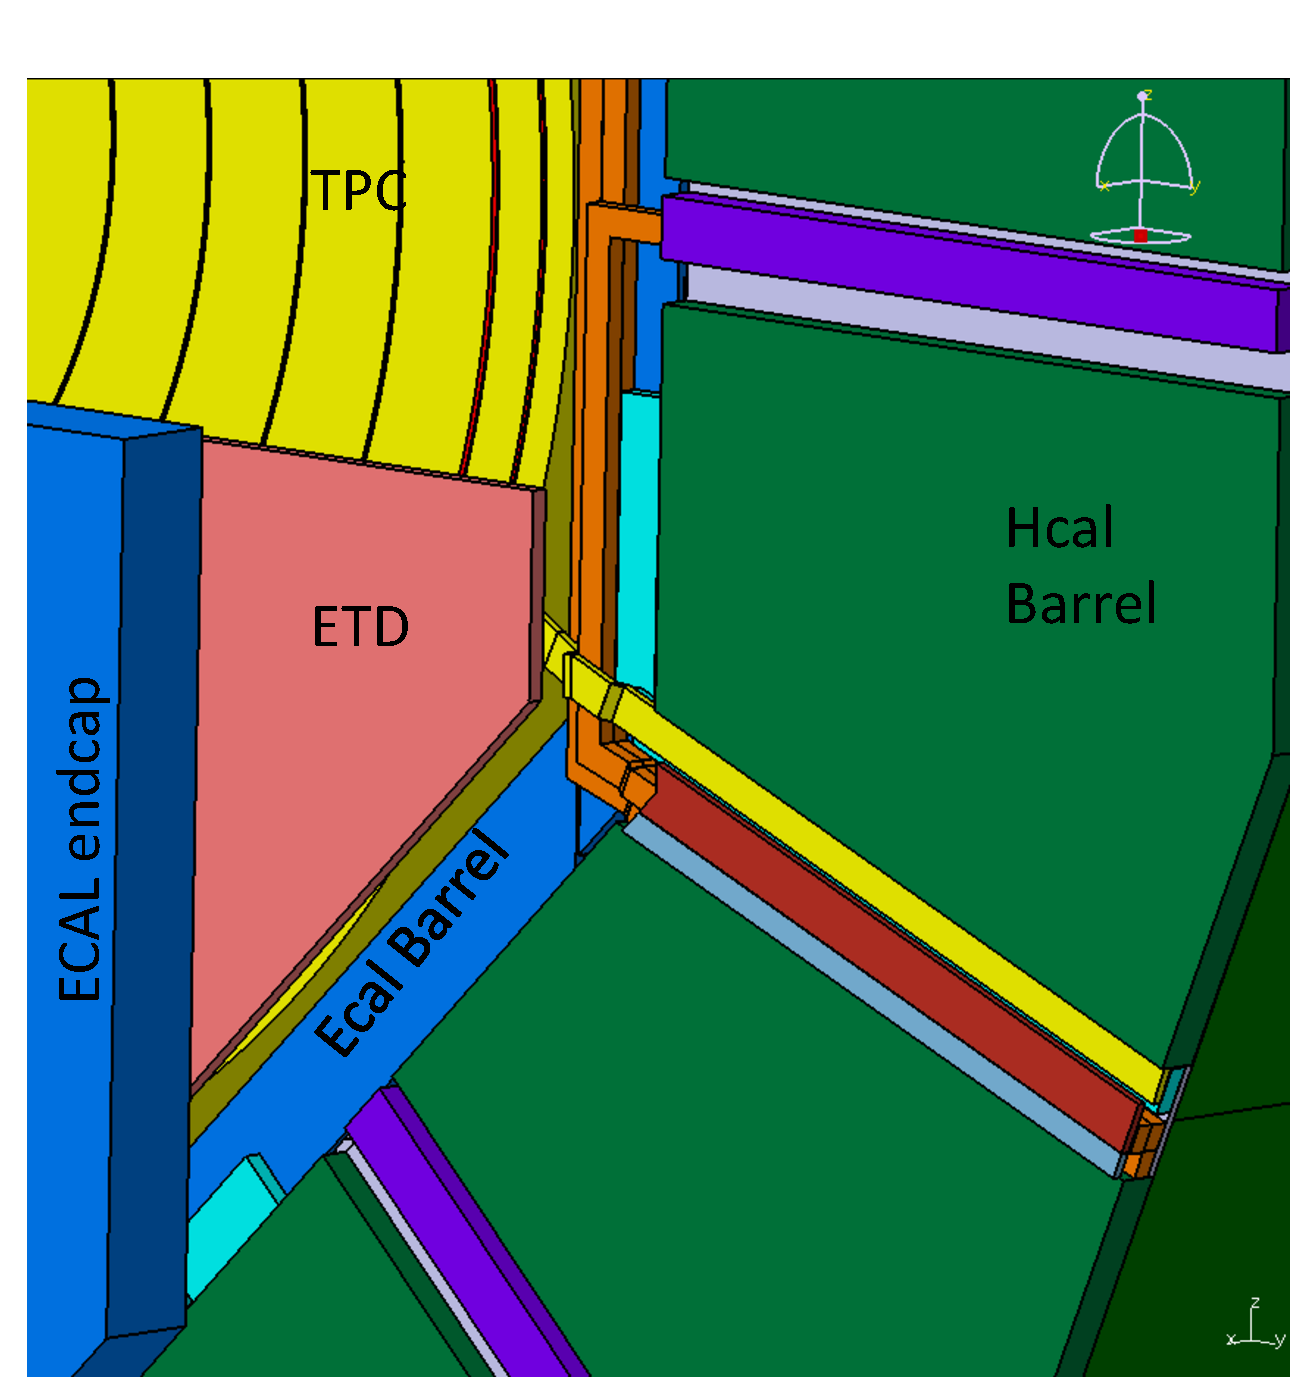
\includegraphics[width=0.7\hsize]{Integration/fig/Barrel_Services.pdf}
    \caption{Service paths on the AHCAL barrel front. The domain tagged "ETD" corresponds to an empty space following removal of the Endcap Tracking Detector from the ILD baseline design (section 5.1.2).}
    \label{ILD:fig:barrel_services}
\end{figure}
\subsubsection{SDHCAL Electrical Services and Cooling}
The SDHCAL barrel detector consists of three or five rings of eight wedge-shaped modules in the Videau configuration. As the active layers are installed from the outside of the barrel structures, access requires the removal of the respective barrel rings from the detector solenoid. The cables and cooling services run on the outside of each module to the barrel front face, as shown in Figure~\ref{ILD:fig:sdcal_module_services}. The SDHCAL services are routed around the detector solenoid to the outside. The services of the inner detector, the ECAL and the TPC can be routed on the front side of the SDHCAL barrel detector, as shown in Figure~\ref{ILD:fig:sdhcal_barrel_services}.
\begin{figure}[h!]
    \centering
        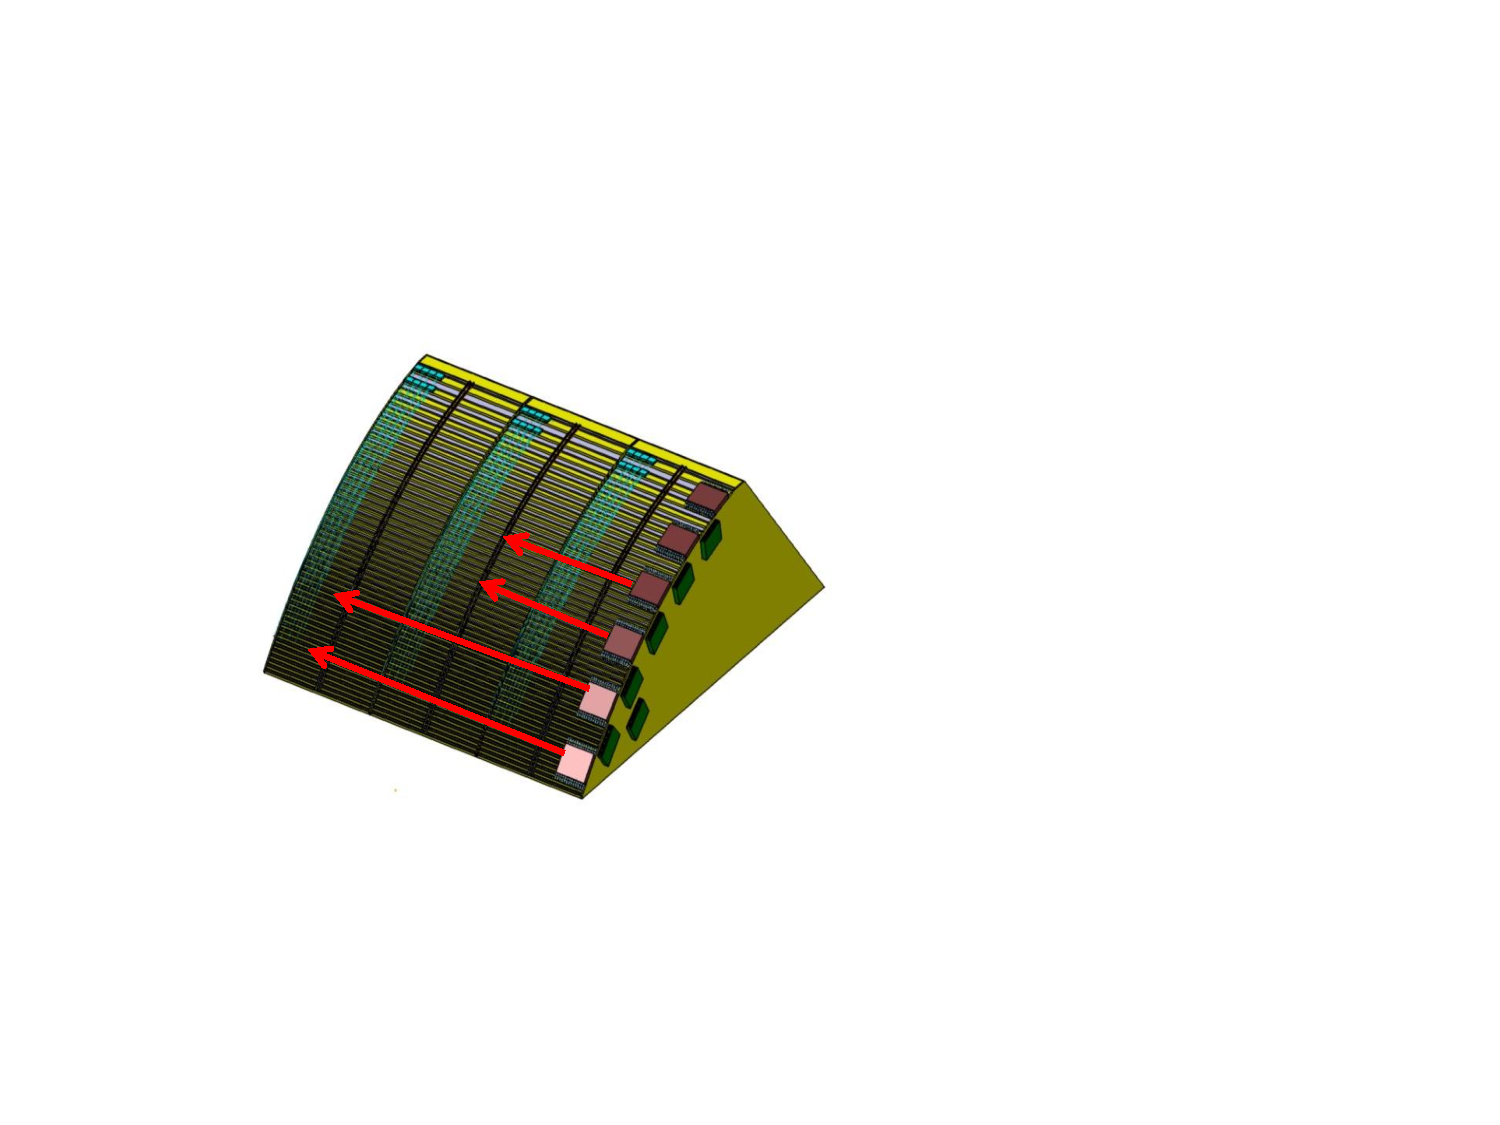
\includegraphics[width=0.8\hsize]{Integration/fig/SDHCAL_Module_Services.pdf}
    \caption{SDHCAL module with readout boards, cables and cooling lines.}
    \label{ILD:fig:sdcal_module_services}
\end{figure}
\begin{figure}[h!]
    \centering
        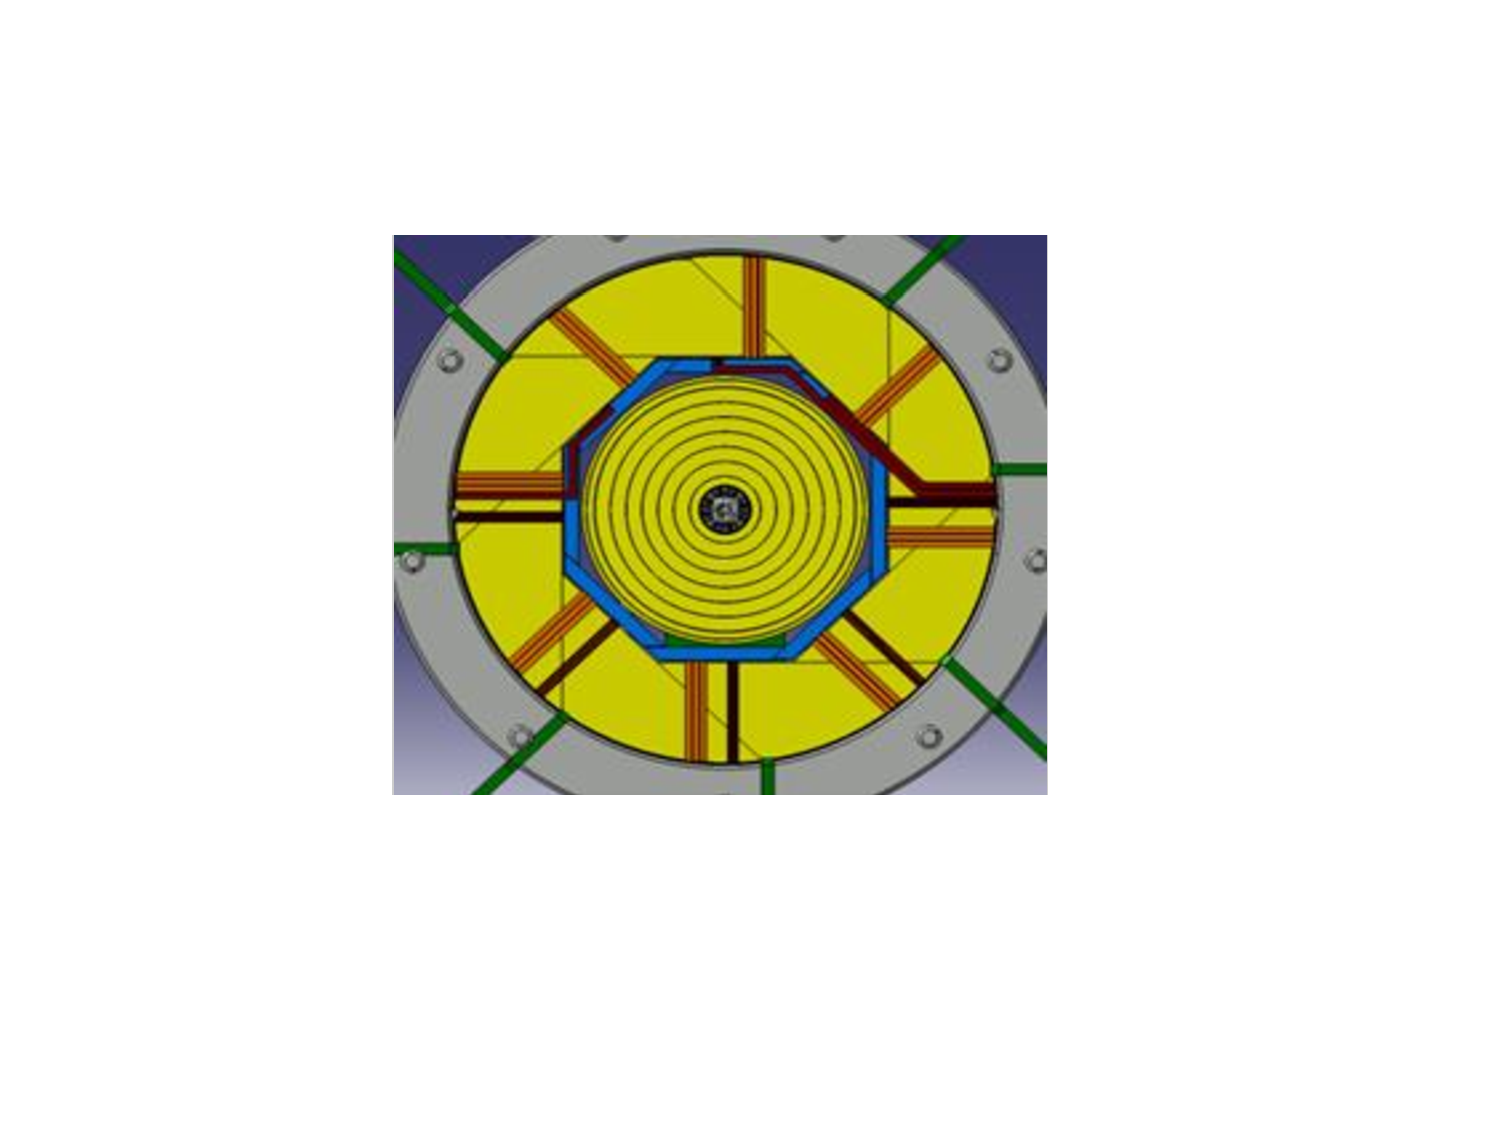
\includegraphics[width=0.8\hsize]{Integration/fig/SDHCAL_Barrel_Services.pdf}
    \caption{Service paths on the SDHCAL barrel front.}
    \label{ILD:fig:sdhcal_barrel_services}
\end{figure}

%\subsection{Yoke/Muon Integration}

\subsection{Very Forward System Integration}
The very forward systems, BeamCal, LumiCal and LHCal, are carried by the support structure for the final focus quadrupole QD0. Figure~\ref{ILD:fig:vfs_integration} shows the mechanical layout and the conceptual service paths of the forward calorimeters.
\begin{figure}[h!]
    \centering
    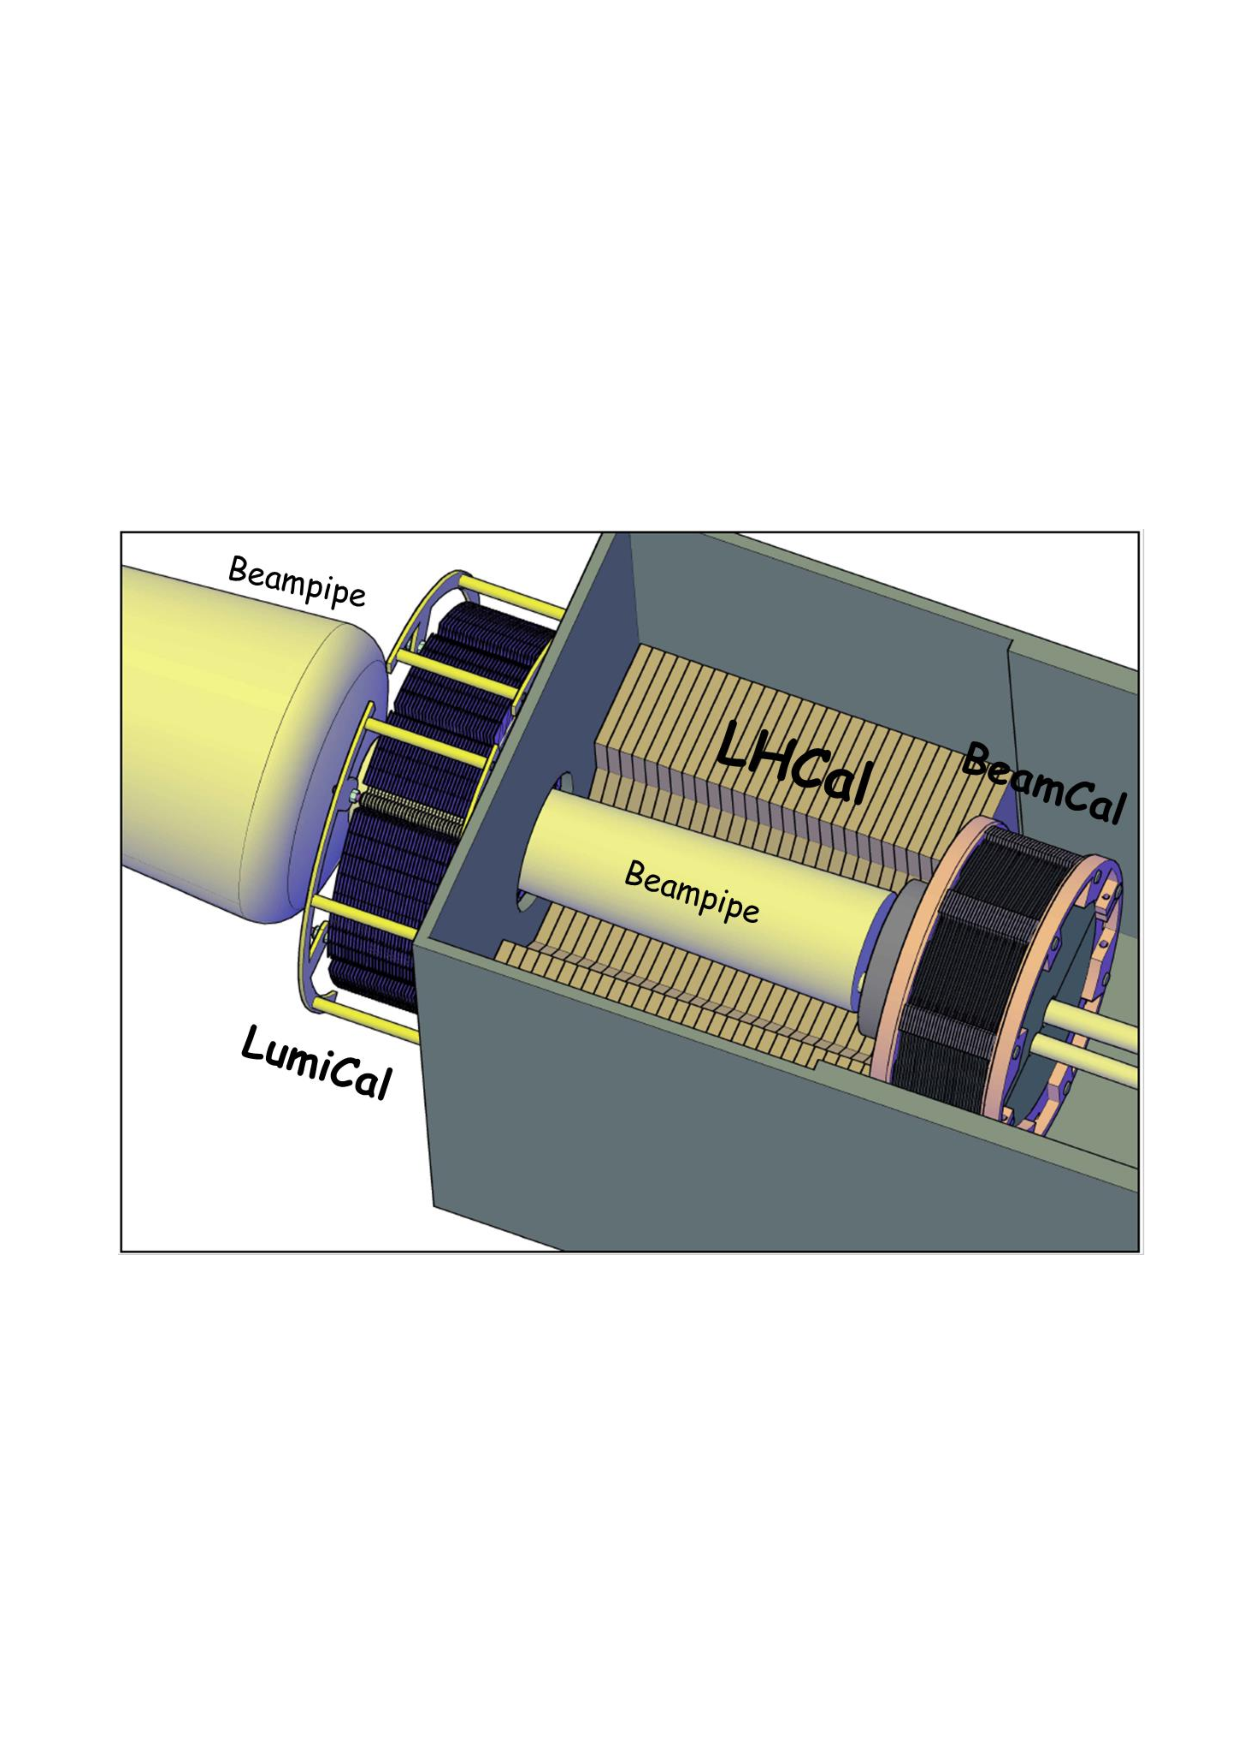
\includegraphics[width=0.45\hsize]{Integration/fig/VFS_Design.pdf}
        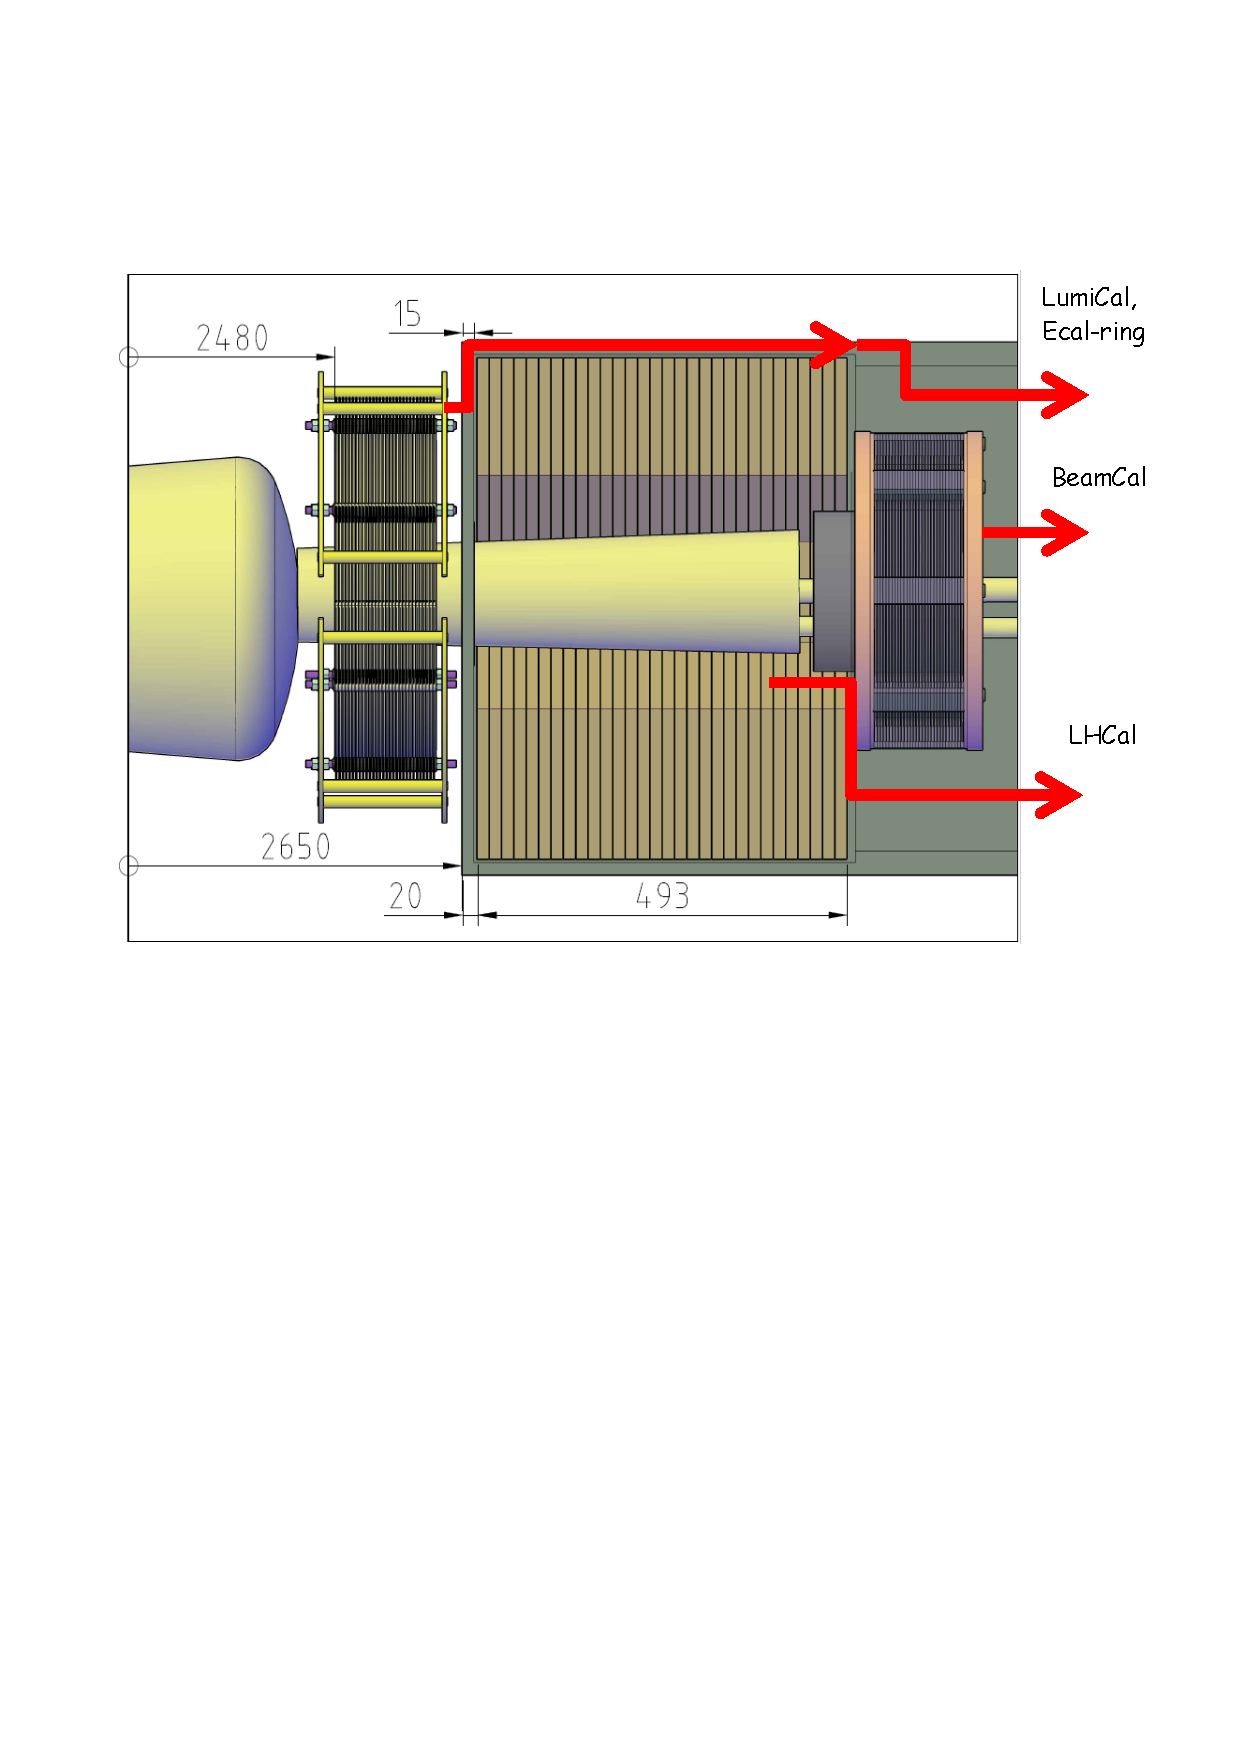
\includegraphics[width=0.45\hsize]{Integration/fig/VFS_Services.pdf}
    \caption{Design of the very forward systems with indication of service and cable paths~\cite{ild:bib:VFS_ICD}.}
    \label{ILD:fig:vfs_integration}
\end{figure}